\documentclass[12pt]{article}
\usepackage[english]{babel}
\usepackage[utf8x]{inputenc}
\usepackage{amsmath}
\usepackage{graphicx}
\usepackage{pdfpages}
\usepackage[colorinlistoftodos]{todonotes}
\usepackage{rotating}

\begin{document}

\begin{titlepage}

\newcommand{\HRule}{\rule{\linewidth}{0.5mm}} % Defines a new command for the horizontal lines, change thickness here

\center % Center everything on the page


\textsc{\LARGE ECE241 Project}\\[1.5cm] % Name of your university/college
\textsc{\large University of Toronto}\\[0.5cm] % Minor heading such as course title

\HRule \\[0.4cm]
{ \huge \bfseries Super Mario Bros.}\\[0.4cm] % Title of your document
\HRule \\[1.5cm]
 

\begin{minipage}{0.4\textwidth}
\begin{flushleft} \large
\emph{Authors:}\\
Hannah \textsc{Brooks}\\
1004868501 \\
Wasif \textsc{Butt}\\
1004879303
\end{flushleft}
\end{minipage}
~
\begin{minipage}{0.4\textwidth}
\begin{flushright} \large
\emph{Teaching Assistant:} \\
Ciaran \textsc{Bannon}\\

\emph{Practical Session:} \\ 
PRA0102 - BA3145 
\end{flushright}
\end{minipage}\\[2cm]


{\large December 2, 2019}\\[2cm] % Date, change the \today to a set date if you want to be precise
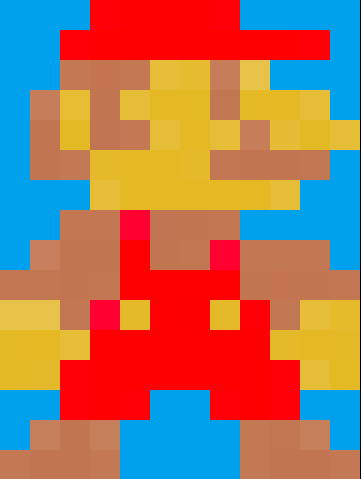
\includegraphics[scale=0.2]{mario.png}

 
%----------------------------------------------------------------------------------------
\end{titlepage}

\section{Introduction}
For our final project we wanted a task that was flexible in terms of complexity, so that features could be compounded or simply have the bare minimum, depending on time constrains. We decided to build a replica of the original 8 bit classic NES game, Super Mario Bros. The game includes a title screen and 3 levels. Mario is able to move left and right as well jump, given user input. He is also able to fall down and on to objects. Furthermore the user is able to navigate between the three levels seamlessly. The game utilizes a VGA adapter to display images from ROM onto the 160x120 pixel display, takes movement input from a PS/2 keyboard using a PS/2 driver, plays background music using an Audio Controller, and finally, has a timer on the HEX display to keep track of how long the user has been playing. 

\section{The Design}

\begin{figure}[h!]
\centering
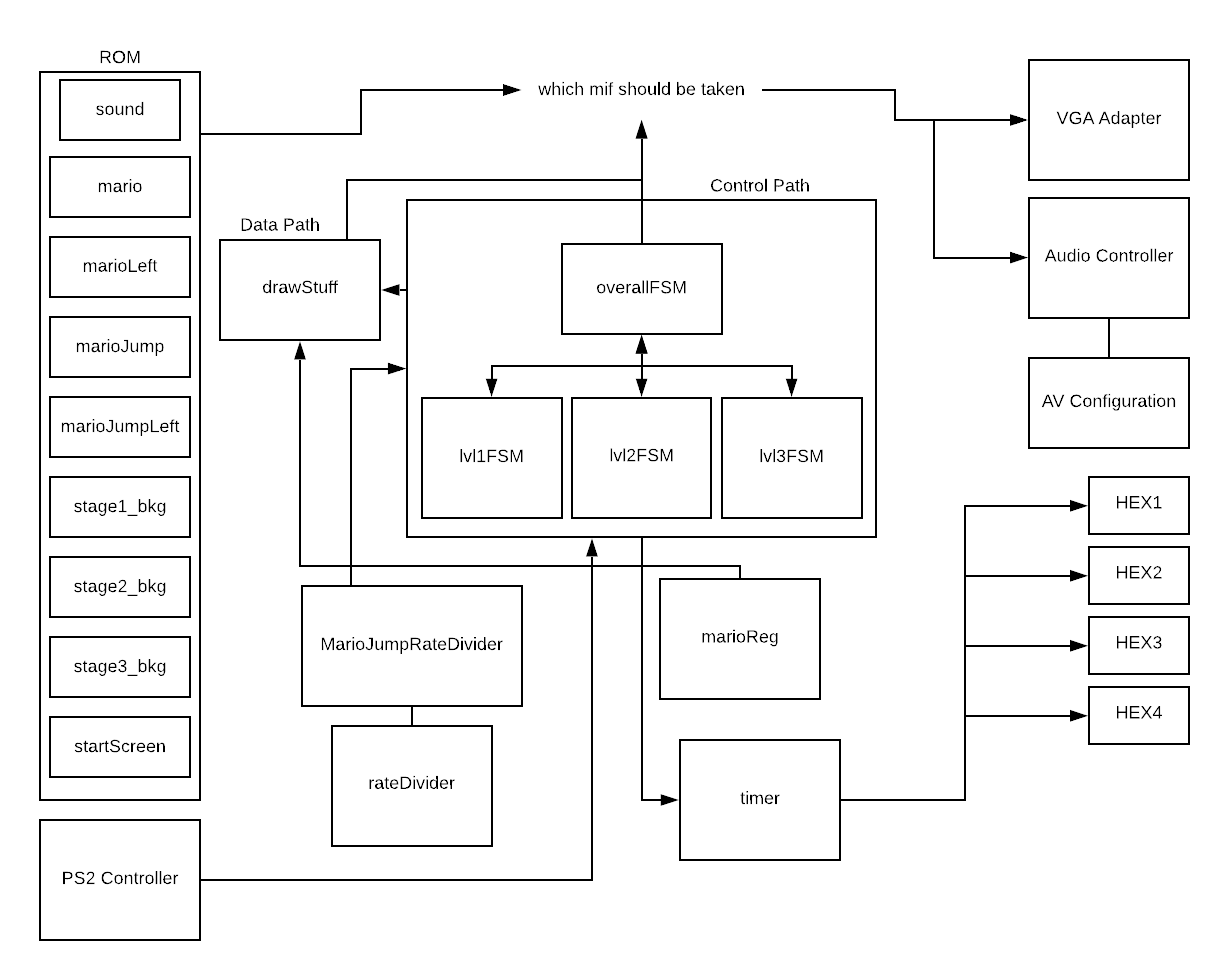
\includegraphics[width=13.5cm]{schematic.png}
\end{figure}

\subsection{Overall Control}
An overall FSM controls which stage Mario is on and each stage has a corresponding FSM to control his movement. Although each level has a separate control path FSM, the game still uses a common data path and register to draw MIFs and to move Mario. For this reason each level-specific FSM has a wait state that requires an enable signal from the overall FSM before it can access these modules. This reduced signal bouncing that caused MIFs to draw incorrectly. The top level module uses FSM outputs to select colour, x position, y position and enable inputs for the VGA adapter. 
\subsection{The Keyboard}
The link between the game and the keyboard uses the PS/2 controller modules and included code provided. We used the \texttt{received\_data} port to check which keys were being pressed (up, down, left, right) as well as any internal combination. The proceeding action was determined based on a combination of the previous signal and the state of the \texttt{received\_data\_en} signal. The data is sent into level-specific FSMs and to Mario's movement register. 
\subsection{The Audio}
Similar to the keyboard functions, the audio was implemented using code provided. The primary modules used were the Audio Controller alongside the configuration module for the chip. The two modules were instantiated with frequencies being read in from a MIF stored in ROM, and passed to both the left and right channels as square waves with different periods. Each note at a different address was played sequentially using an up counter. A total of 1000 notes play on loop as background music. 
\subsection{VGA Adapter / ROM}
In this project, we used a total 8 MIFs, each was stored in ROM. All ROM modules are instantiated and continually read from while their colour outputs are stored in wires. The control path chooses when to assign VGA colour input to a respective wire. Using registers, a memory address input extracts a 12 bit colour that was then passed to the VGA adapter to display at a specified (x, y) location, based upon the data path output. Mario is able to look like he was moving by redrawing the background over all previous images and then redrawing him in a new (x, y) position. All MIFs can be seen at end of section 3.  
\subsection{Mario's Movement}
A user is able to move Mario left, right, and/or up using keyboard inputs. Mario also falls down until he lands on a surface after hitting the peak of his jump. The basic method for moving Mario was to navigate to the correct state in the FSM after input, update the register, erase Mario, then print Mario in the new position once a rate divider sent an enable signal.\\
\\After clicking a key the FSM moves to an ``erase Mario`` state where the background would be redrawn, effectively making Mario disappear. Mario is then redrawn in a new position after 0.2s (left/right) or 0.0002s (jumping/falling). \\
\\A common register is used to keep track of Mario's (x, y) position on the VGA screen as well as increment/decrement his position depending on the corresponding directional input. The register also checks for boundary and ground conditions by testing where Mario's position was relative to our specified objects on the background. Additionally, for Mario to jump the FSM loops between erasing and redrawing Mario until a counter reaches 22, corresponding to the amount of y pixels his position had moved. If Mario is not on a surface (as identified in the register) the FSM changes states immediately to make him fall until he landed on a surface - this is done without any input from a user. Conditions for movement while falling were also added within the register so that a user can move Mario as he fell, making the game feel more dynamic. 

\section{Report on Success}
At the initial meeting, we set out three key elements we wanted the game to reflect: drawing elements, moving elements, and interacting with elements - each corresponding to one milestone per week. In this project we were successfully able to draw all images given input as well as move Mario in all directions. Mario was also able to interact with certain elements of the each level by moving through level screens and interacting with boundaries. However, two main features we were unable to implement due to time constraints were the addition of coins to collect and enemies to kill. All areas that were completed worked to specifications with small bugs, as outlined in section 4.1. All game screens can be seen below. \\

\begin{wrapfigure}
  \centering
  \begin{minipage}[b]{0.5\textwidth}
    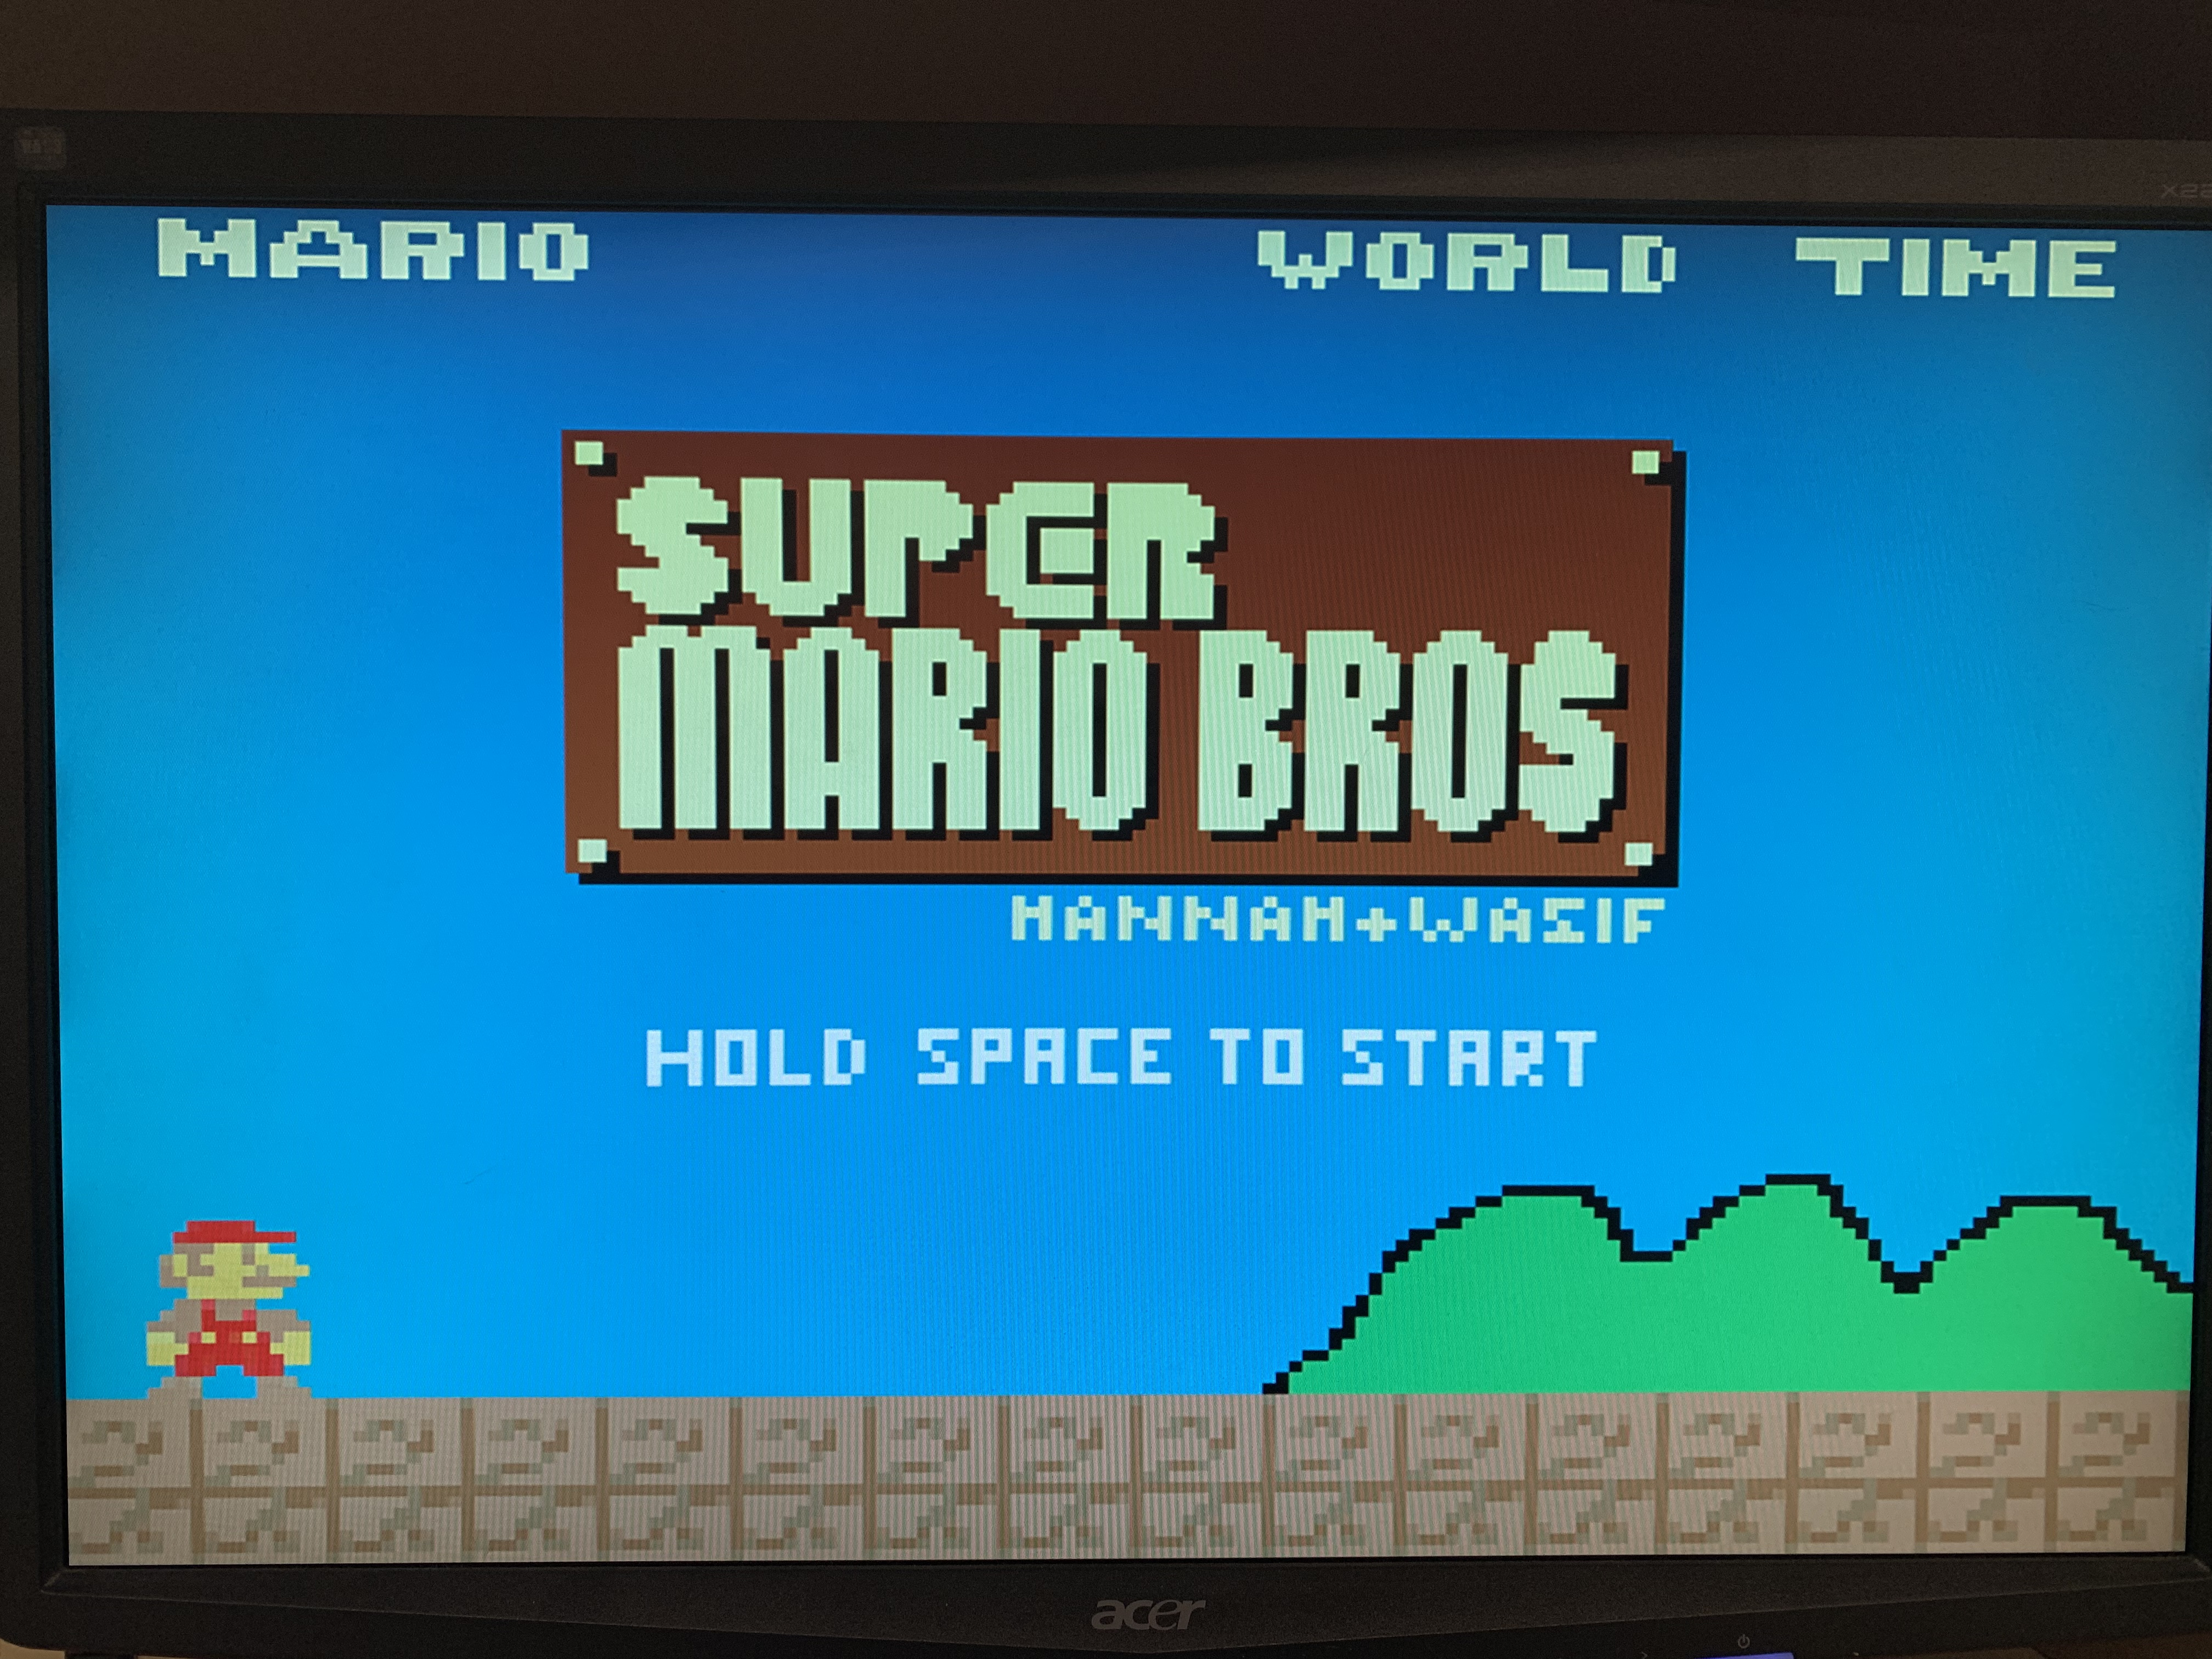
\includegraphics[width=\textwidth]{IMG_1886.jpg}
  \end{minipage}
  \begin{minipage}[b]{0.5\textwidth}
    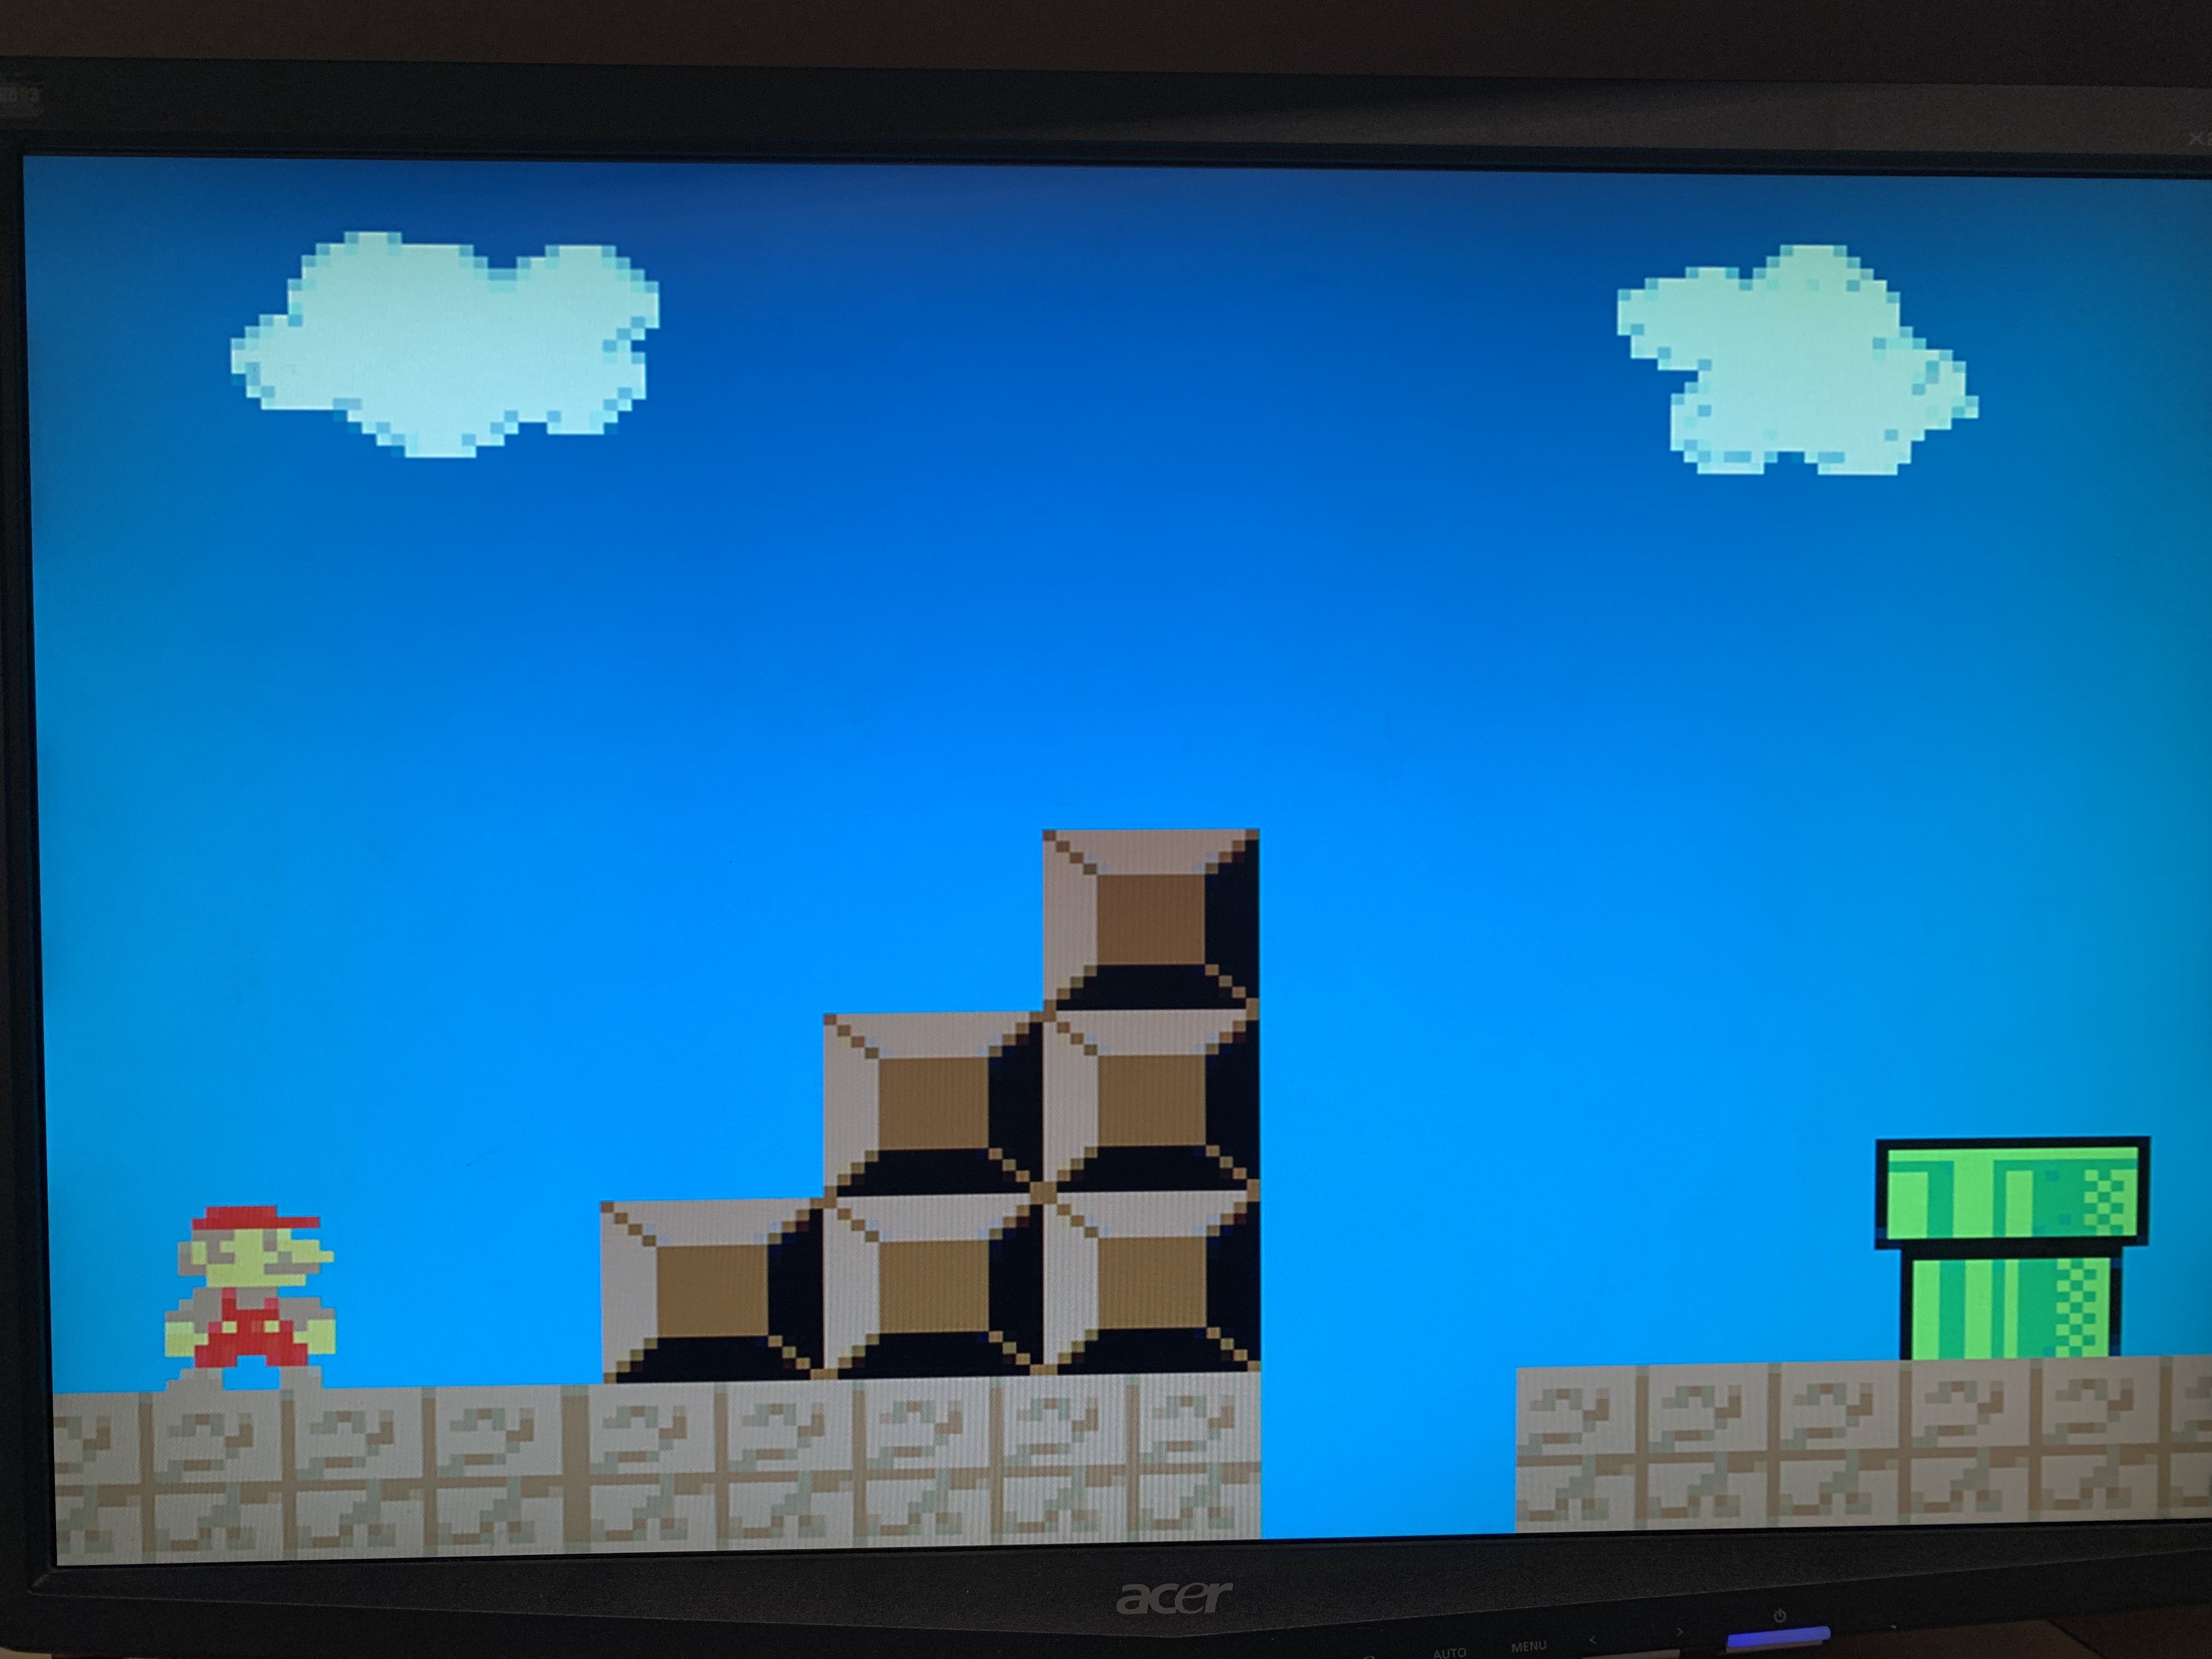
\includegraphics[width=\textwidth]{IMG_1887.jpg}
  \end{minipage}
\end{wrapfigure}
\begin{wrapfigure}
  \centering
  \begin{minipage}[b]{0.5\textwidth}
    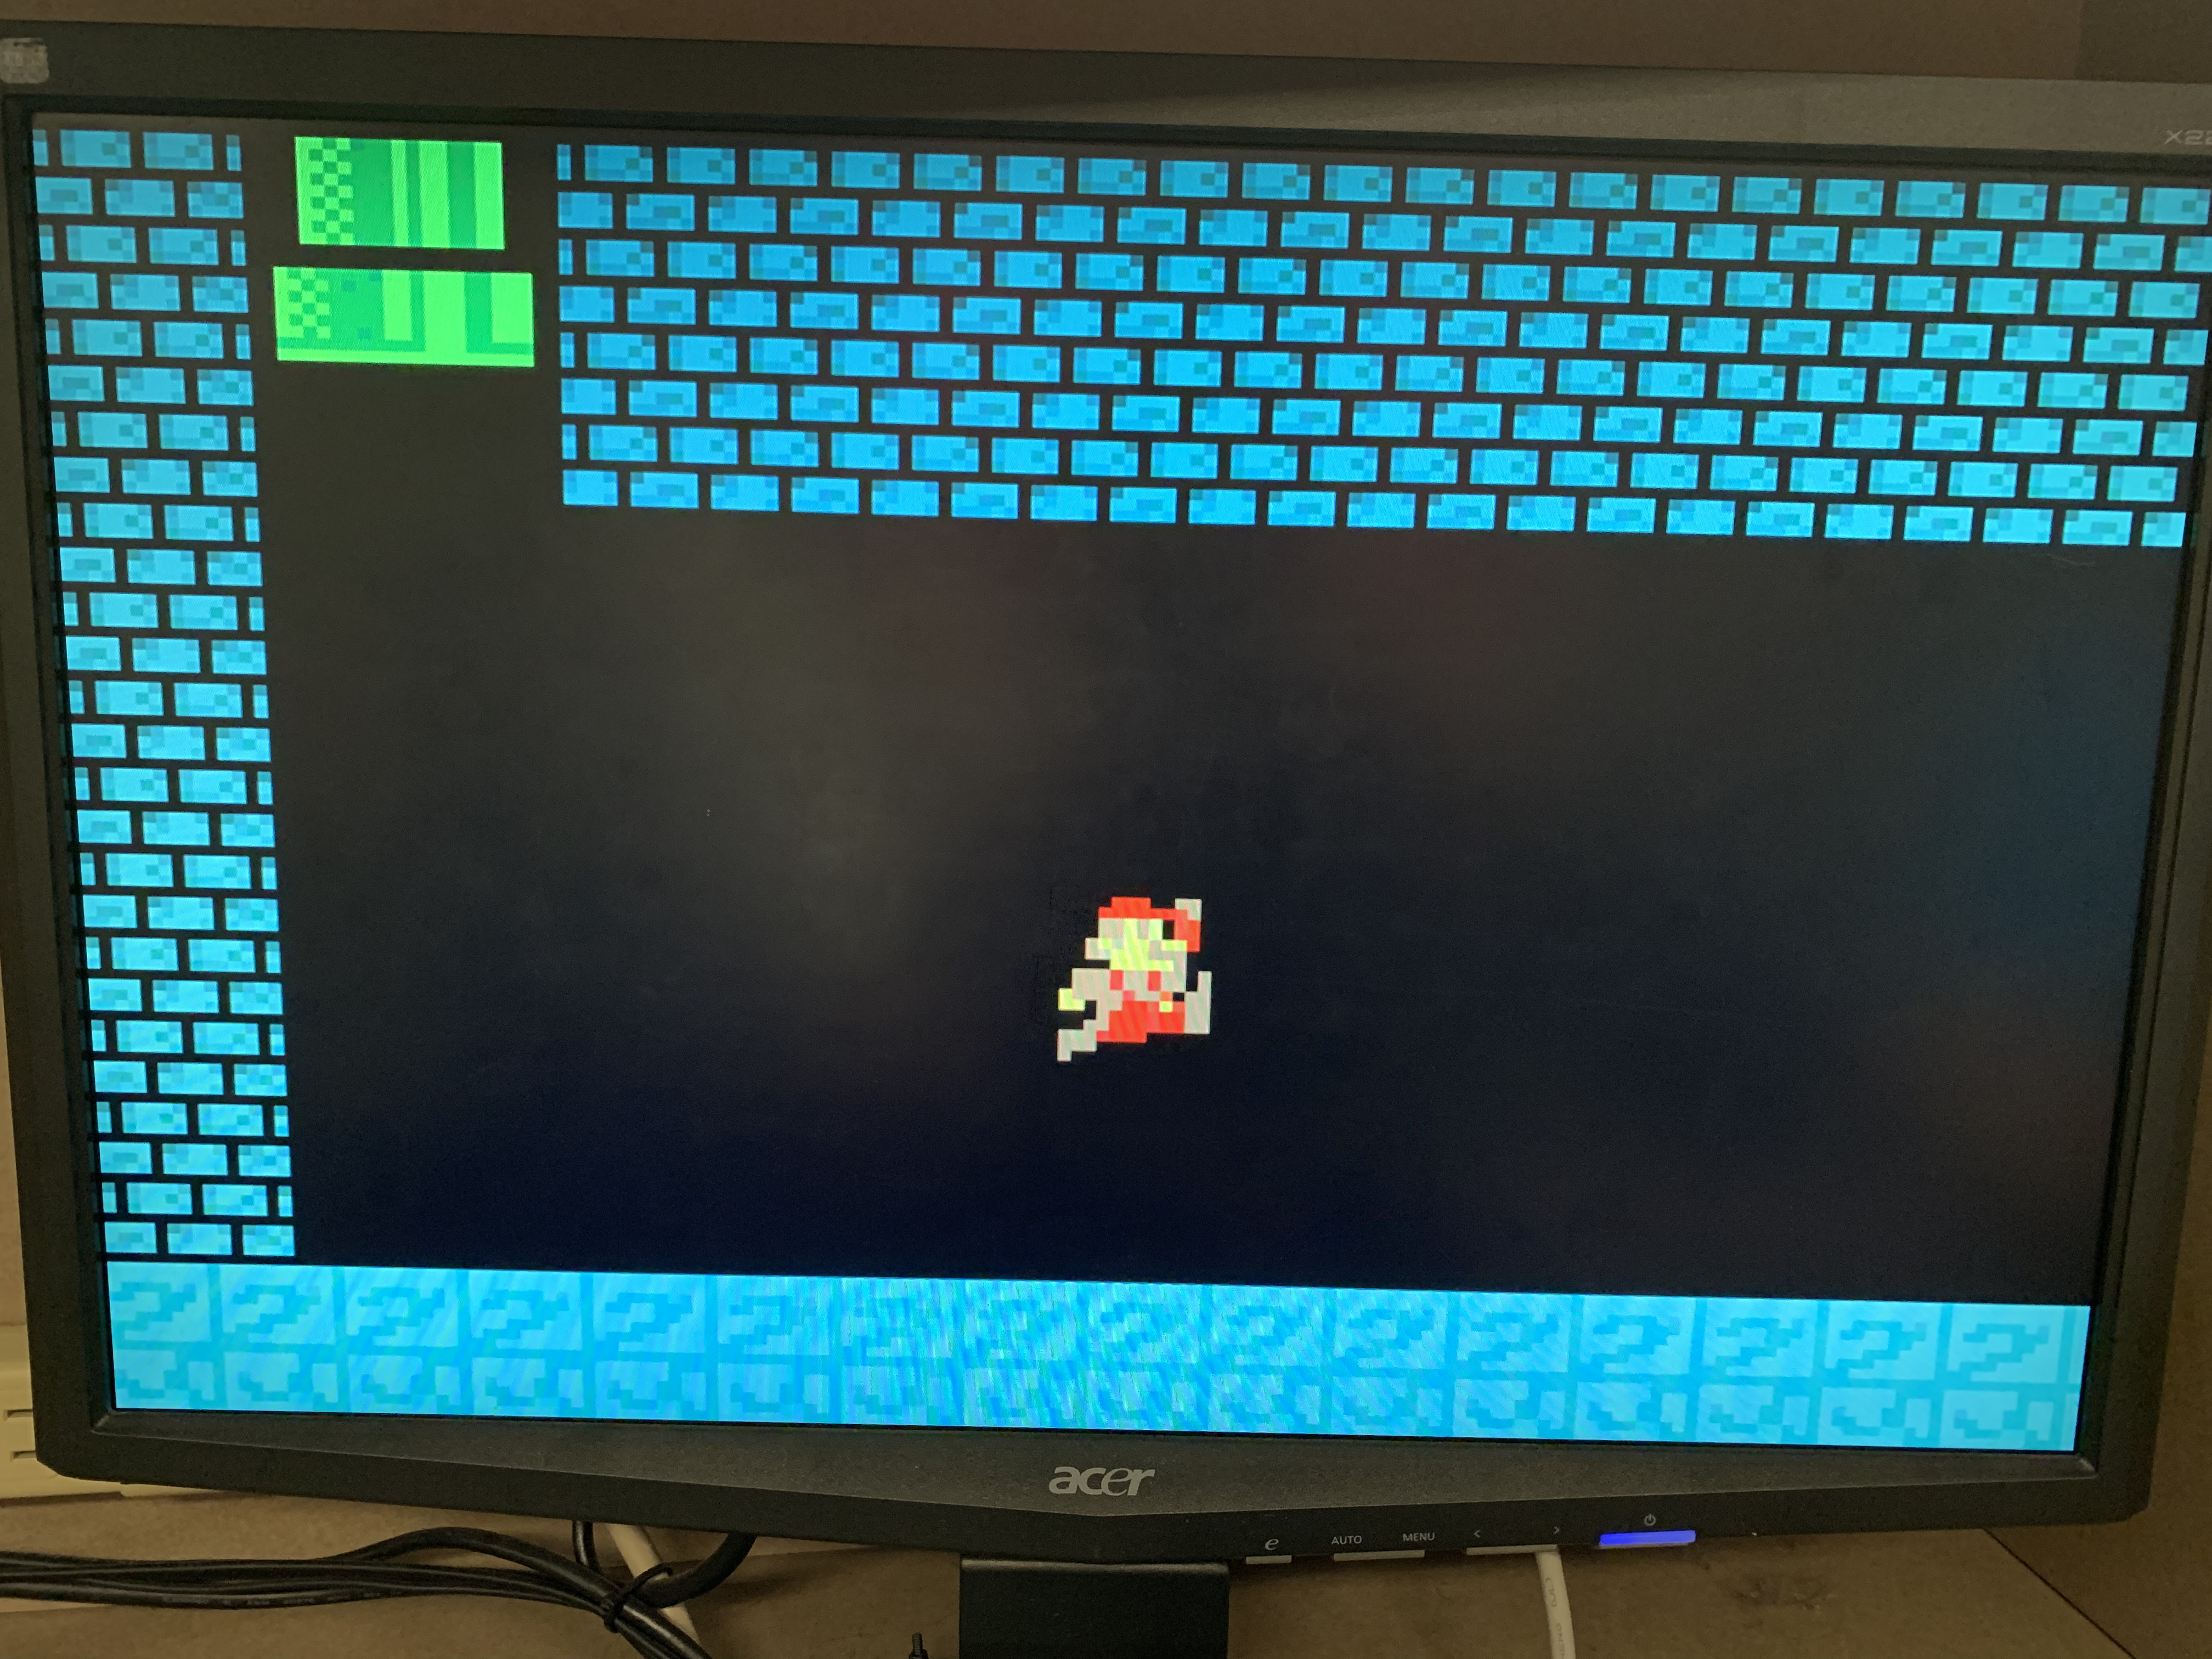
\includegraphics[width=\textwidth]{IMG_1891.jpg}
  \end{minipage}
  \begin{minipage}[b]{0.5\textwidth}
    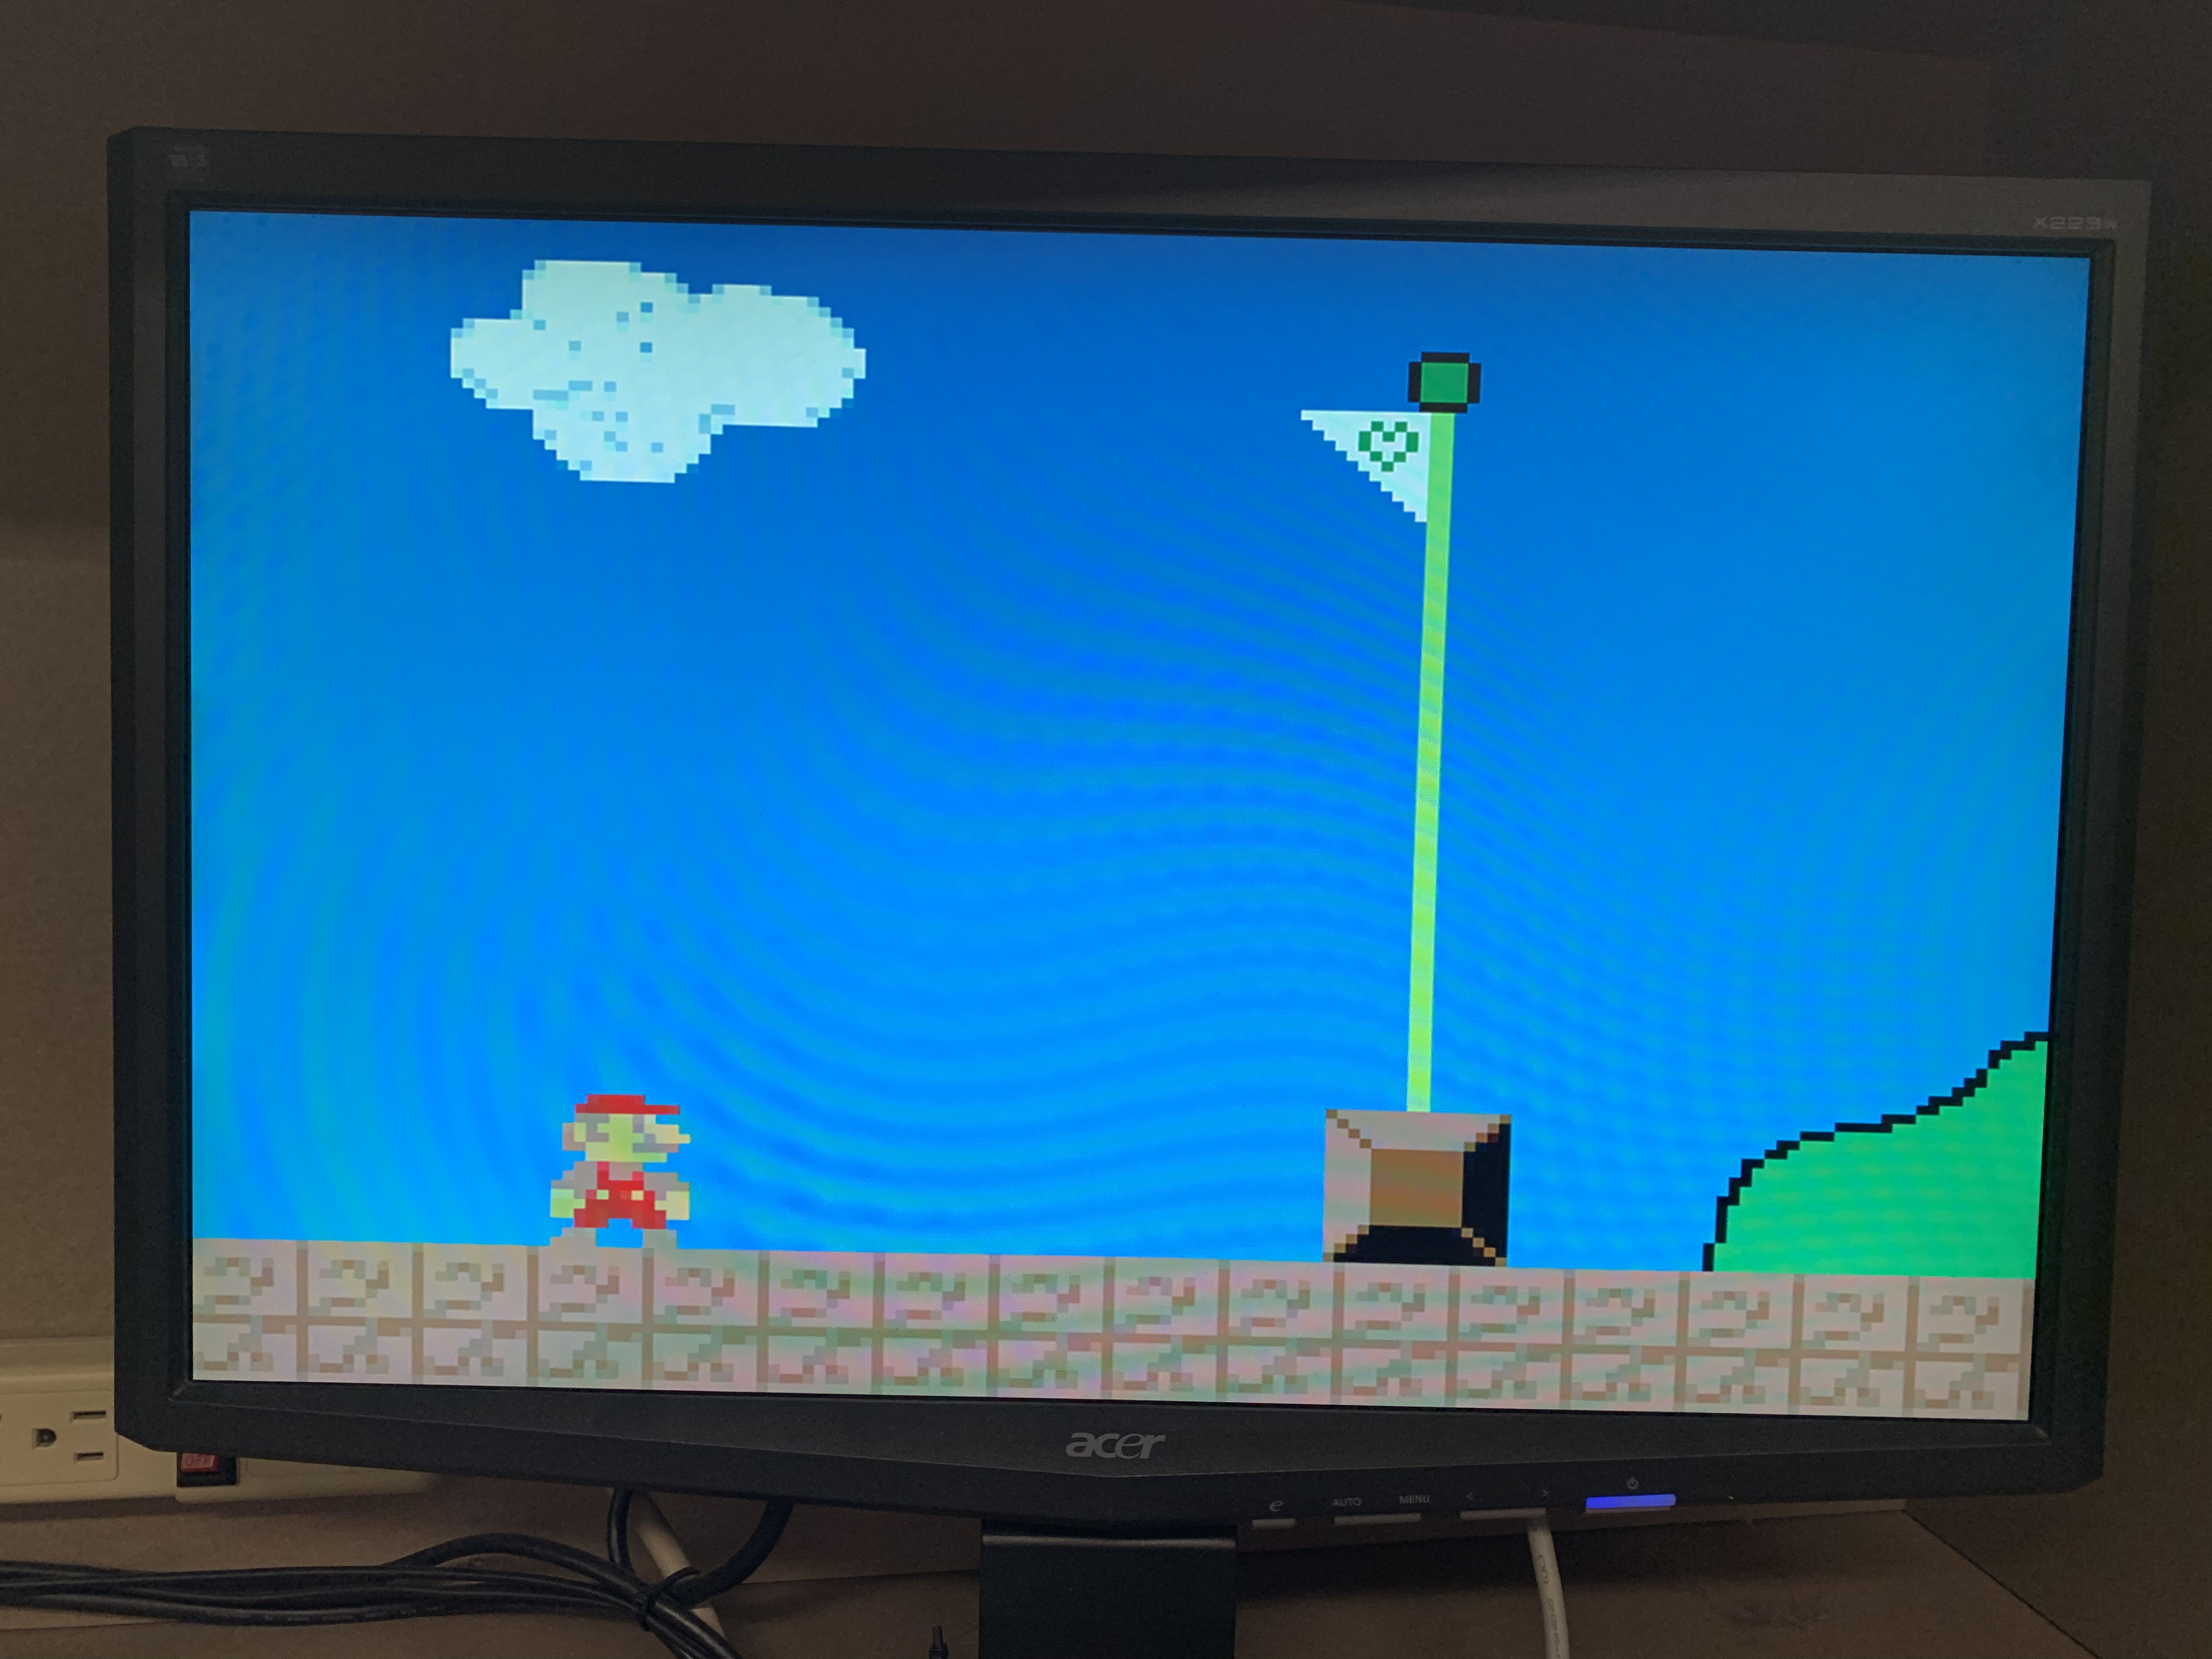
\includegraphics[width=\textwidth]{IMG_1892.jpg}
  \end{minipage}
\end{wrapfigure}


\section{Areas of Improvement}
\subsection{Bugs}
One major bug was the random behaviour of Mario's movement when more than one key was pressed on the PS/2 keyboard. Mario would be able to move through the specified boundaries, something that would not happen if only one key was used at a time to move. The problem is most likely due to the nature of cascading \textbf{if} statements within the register, such that Mario's position is incremented before a boundary condition is checked for because there are two different input arguments that may cause the FSM to go to a state the register was not expecting/not in sync with. Timing analysis to ensure everything was in sync would have fixed this bug. Furthermore, if Mario fell through a hole in level 1 and died the level would switch back to the start screen but the user would no longer be able to play the game again as intended. This is most likely caused by the FSMs resetting incorrectly, which could not be fixed due to time constraints of the project. 
\subsection{Building Blocks}
If we were to work on this project for another week some things that we we would like to add, include: coin collection, enemies, more dynamic animations and more levels. For the coin, we would have liked to have it appear in the Underworld and have \texttt{HEX5} and \texttt{HEX6} keep track of coins collected, this feature was cut due to complexity and time constraints. On the same note, during the second milestone we had both Mario running in the Overworld and the Goomba going back and forth in the Underworld, but did not have success in implementing the two projects together. For both of these, earlier incorporation would have made the merge easier. Further, an additional interesting aspect that would have made this project more dynamic would have been animations. For example, if Mario kills a Goomba, have the Goomba squish and then disappear. Or vice versa, with having Mario die if the Goomba kills him. Lastly, an obvious improvement would have been to have longer levels, more levels or a camera scroll with Mario running. All of these tasks are time consuming but would have been engaging to attempt.
\subsection{Other Road Blocks}
We ran into many road blocks along the course of these three weeks. For example, we ran out of memory using more MIFs than the ROM could hold. This was because we were using 24 bit words instead of the recommended 8 or 12 bit. We downsized all of our MIFs to remedy this problem. We also had issues with version control, where one partner would be working on one instance of the project while another would be working on a different instance and there would be issues with over-writing or difficulties with re-incorporation. We wanted to prevent these issues using Github, or a similar VCS but the computers in the lab are too outdated and do not support these sites running on Internet Explorer. In addition, another problem we encountered was with boundary building. Initially, we had made the decision to determine boundaries using colours, as this made the most intuitive sense. Wherever the background was light blue (in the Overworld) or black (in the Underworld) Mario was allowed to move. However we ended up running into many issues with reading the colours out from memory and the boundaries being created incorrectly. We decided that in order to not waste any more time, we would hard code the boundaries. This was not a big issue, as there was only one instance in the project that needed these explicit boundaries but had our project been any bigger, we would have run into many more issues. 

\section{What We Would Do Differently}
If we were to restart the entire project some things that we would like to do differently would be to use a version control system, incorporate things early and efficiently to prevent hassle in the future and ensure that one piece of code works completely before moving on to another task. As mentioned above, having version control would make it much easier to go back and see what was changed in order to make one part of the project do one thing. Second, we ran into issues where code became more complicated than anticipated which led to incorporation issues. Had we maybe had all components in the project by the second milestone to build up for the last milestone, it may have been easier to have a more complete final project. 

\begin{figure}[h!]
\centering
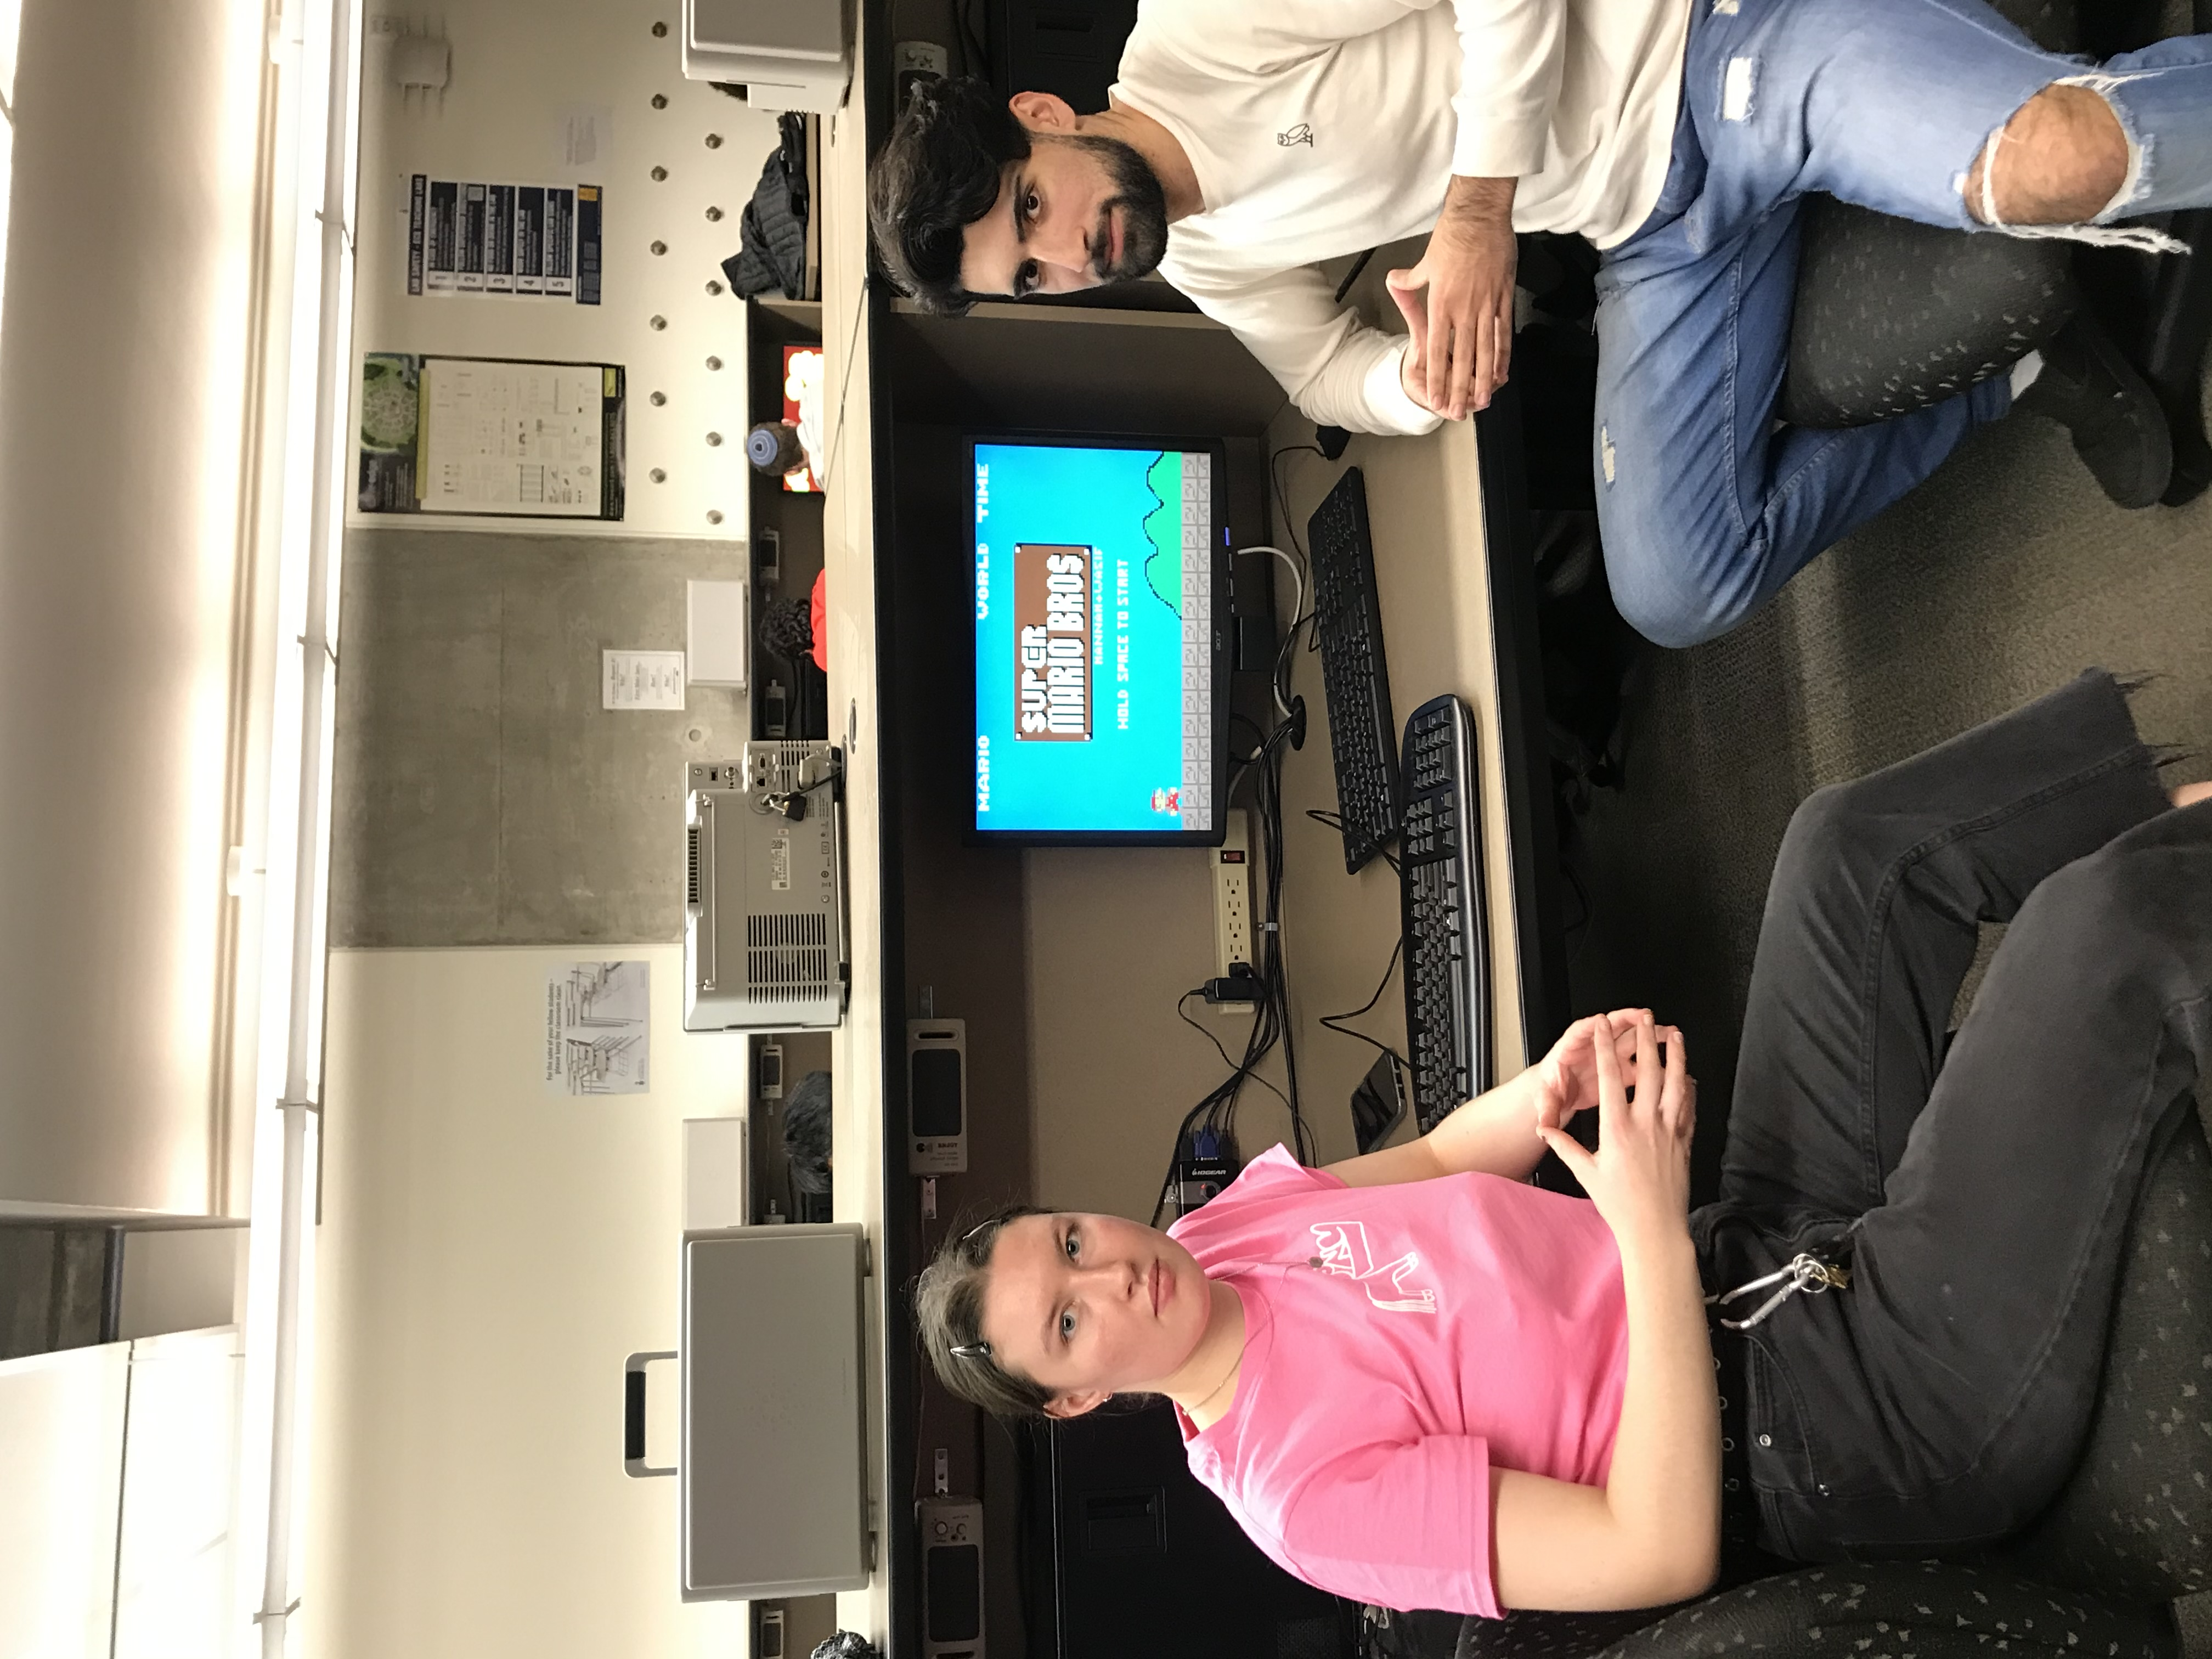
\includegraphics[width=17cm, angle=270]{IMG_1482.jpg}
\caption{Us and our magnificent project}
\end{figure}

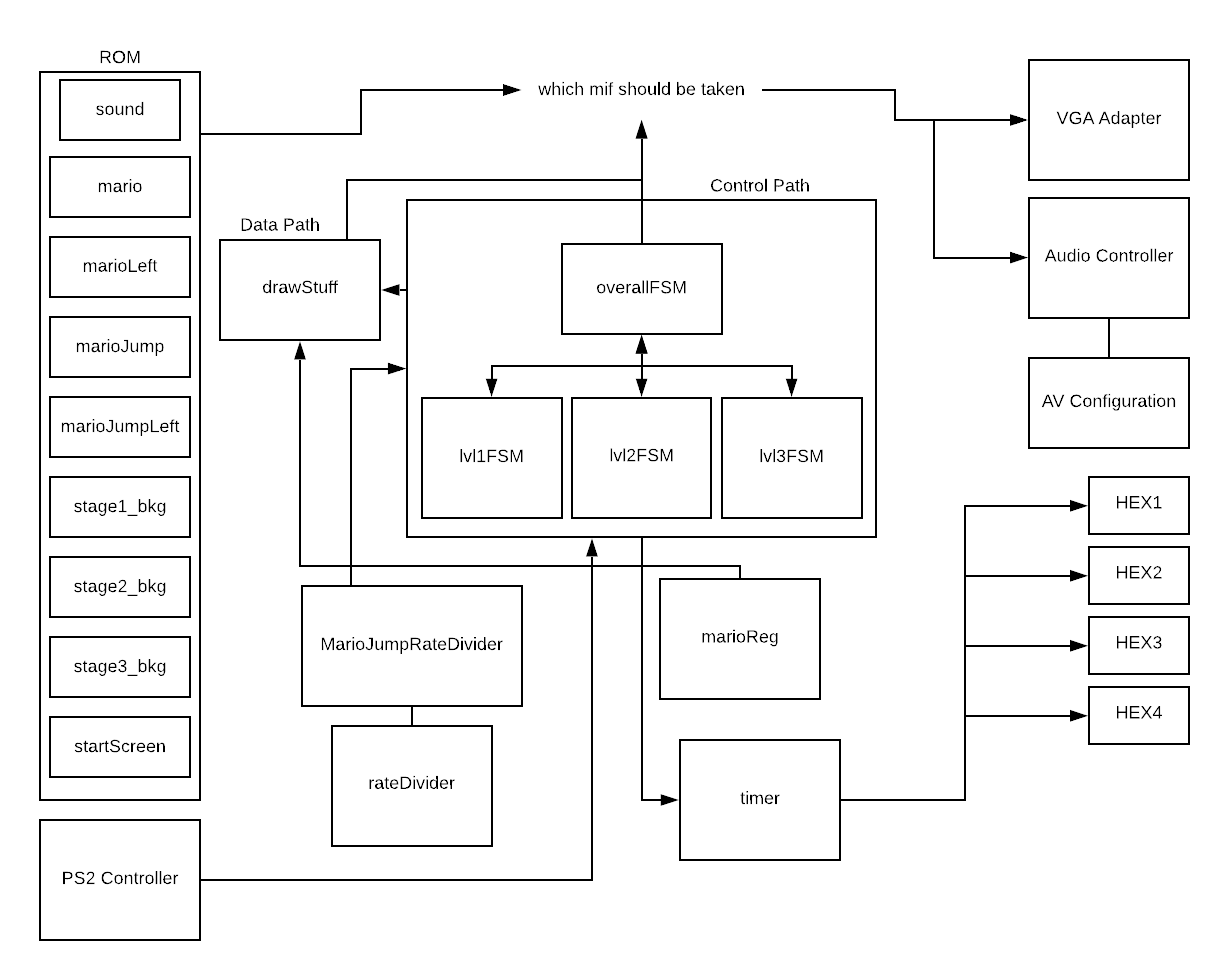
\includepdf[page=-]{schematic}
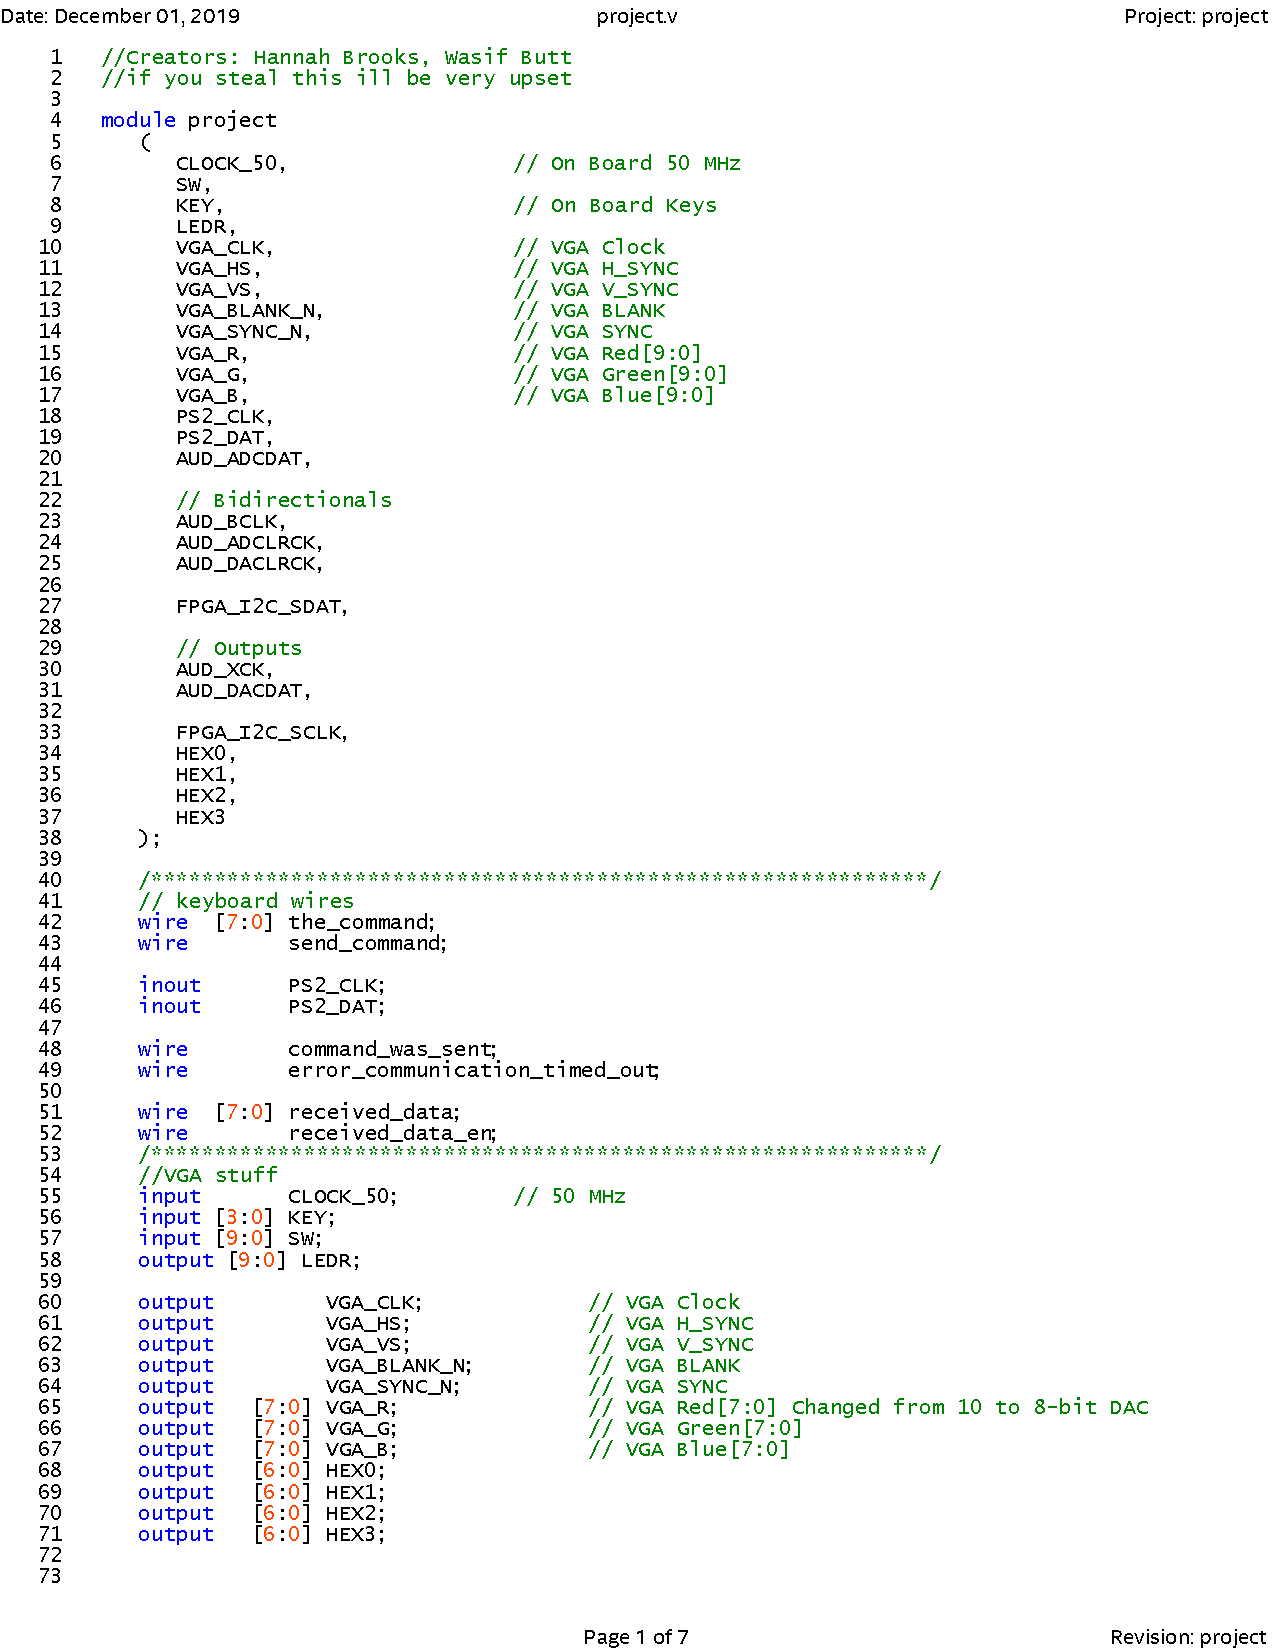
\includepdf[page=-]{codeAsPDF}
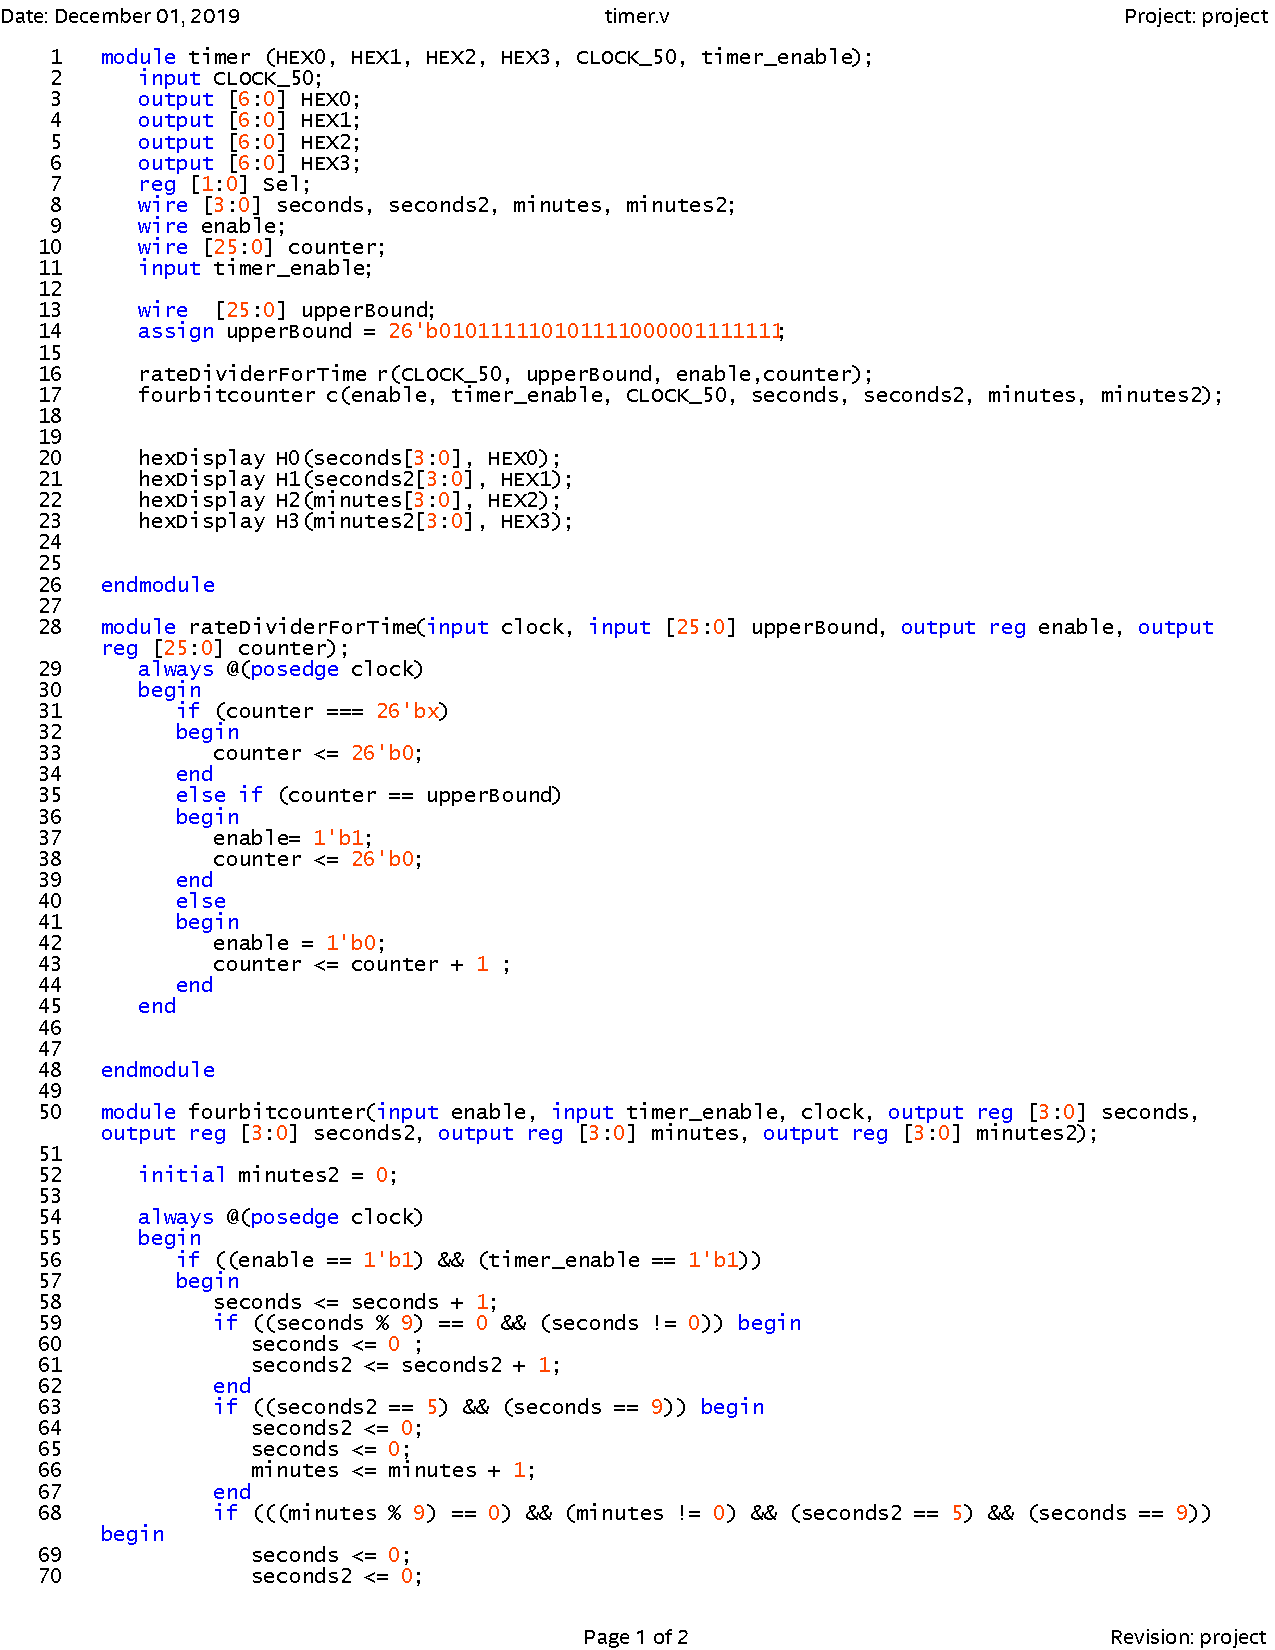
\includepdf[page=-]{1}
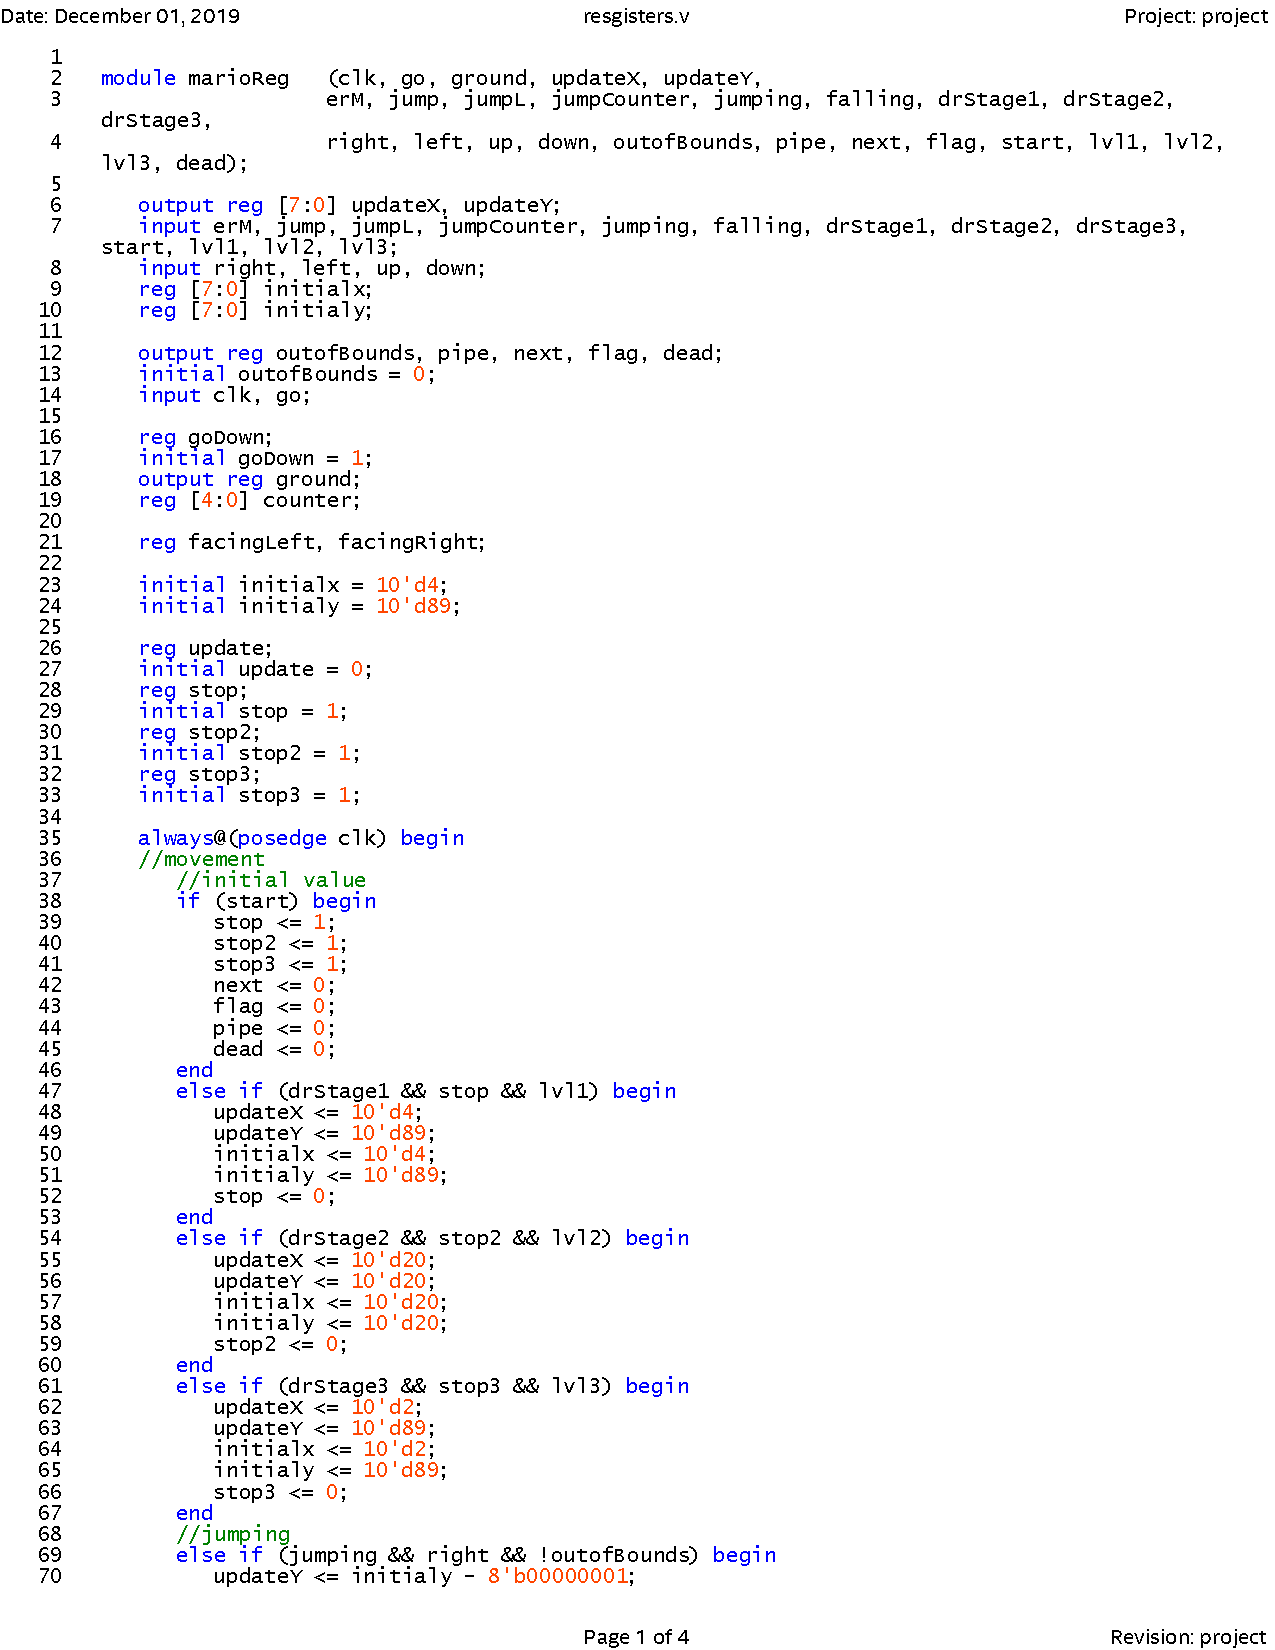
\includepdf[page=-]{2}
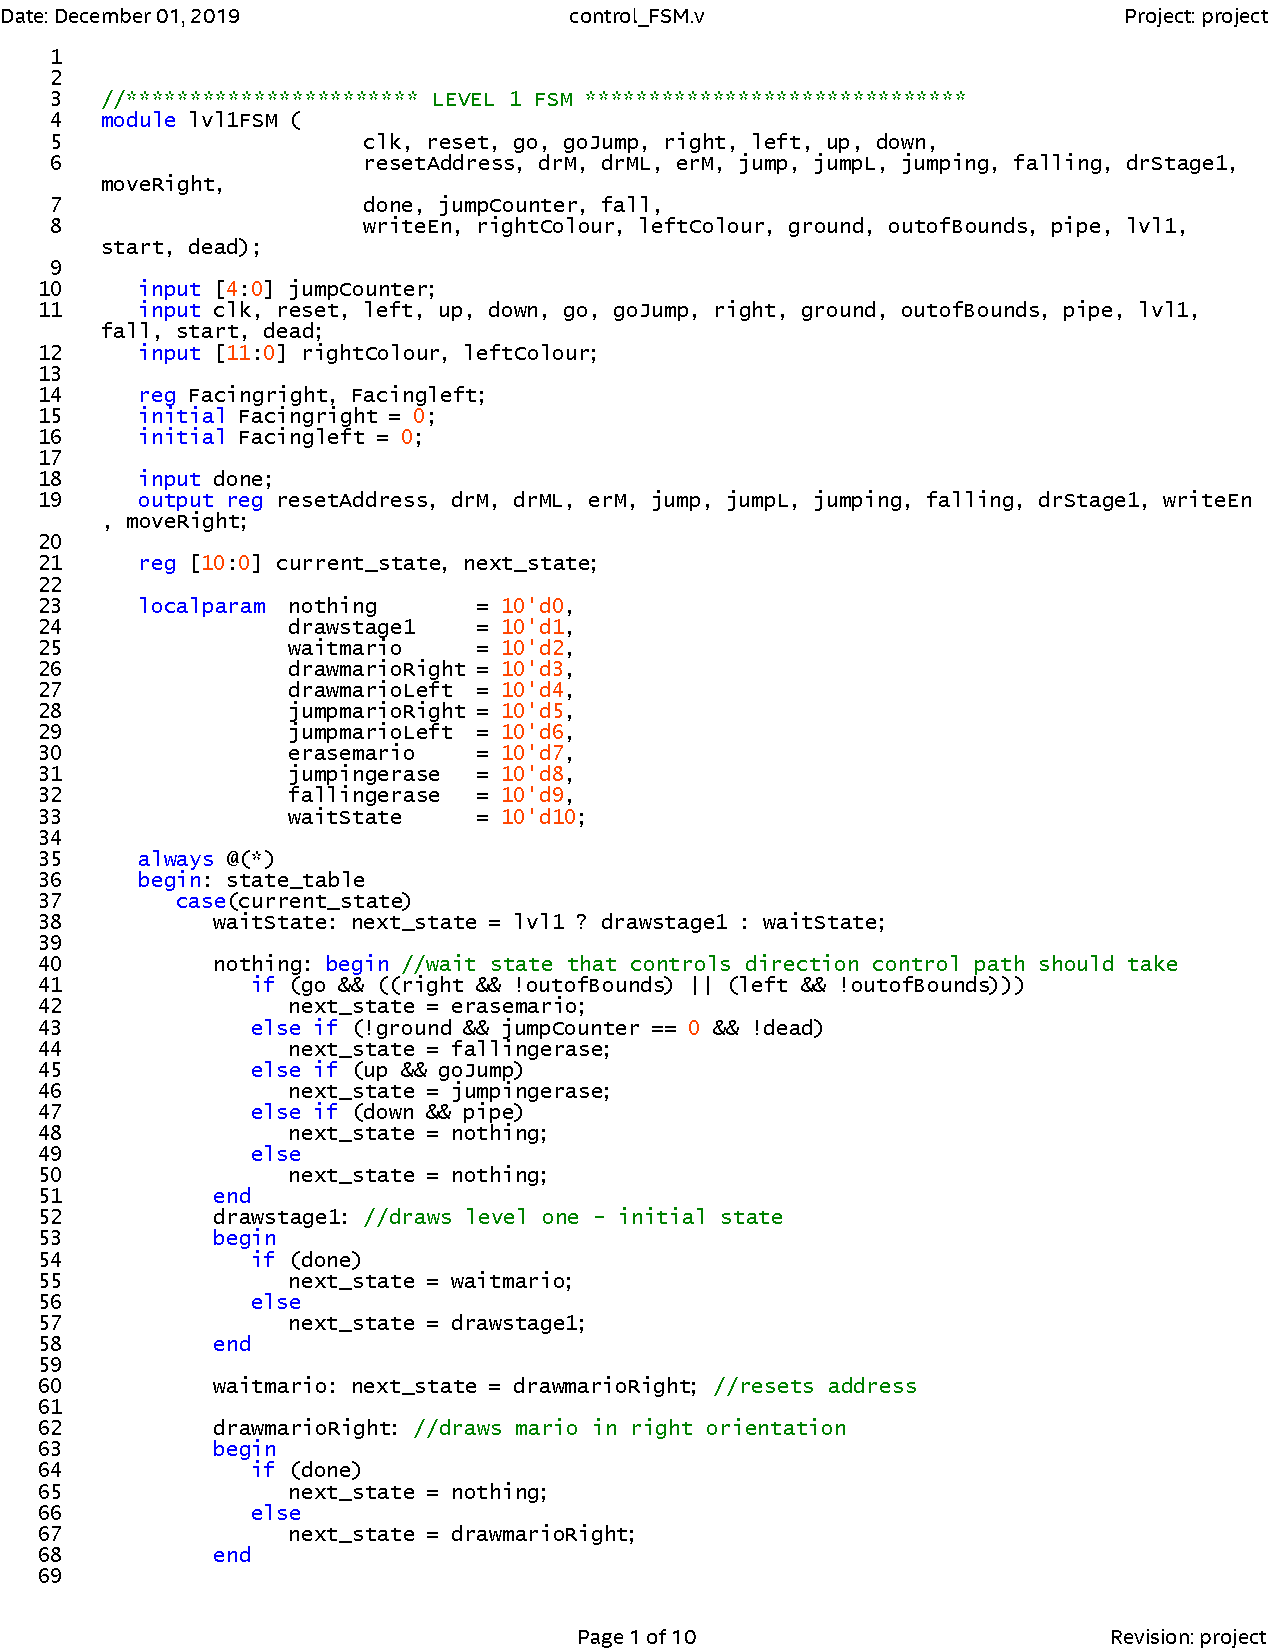
\includepdf[page=-]{3}
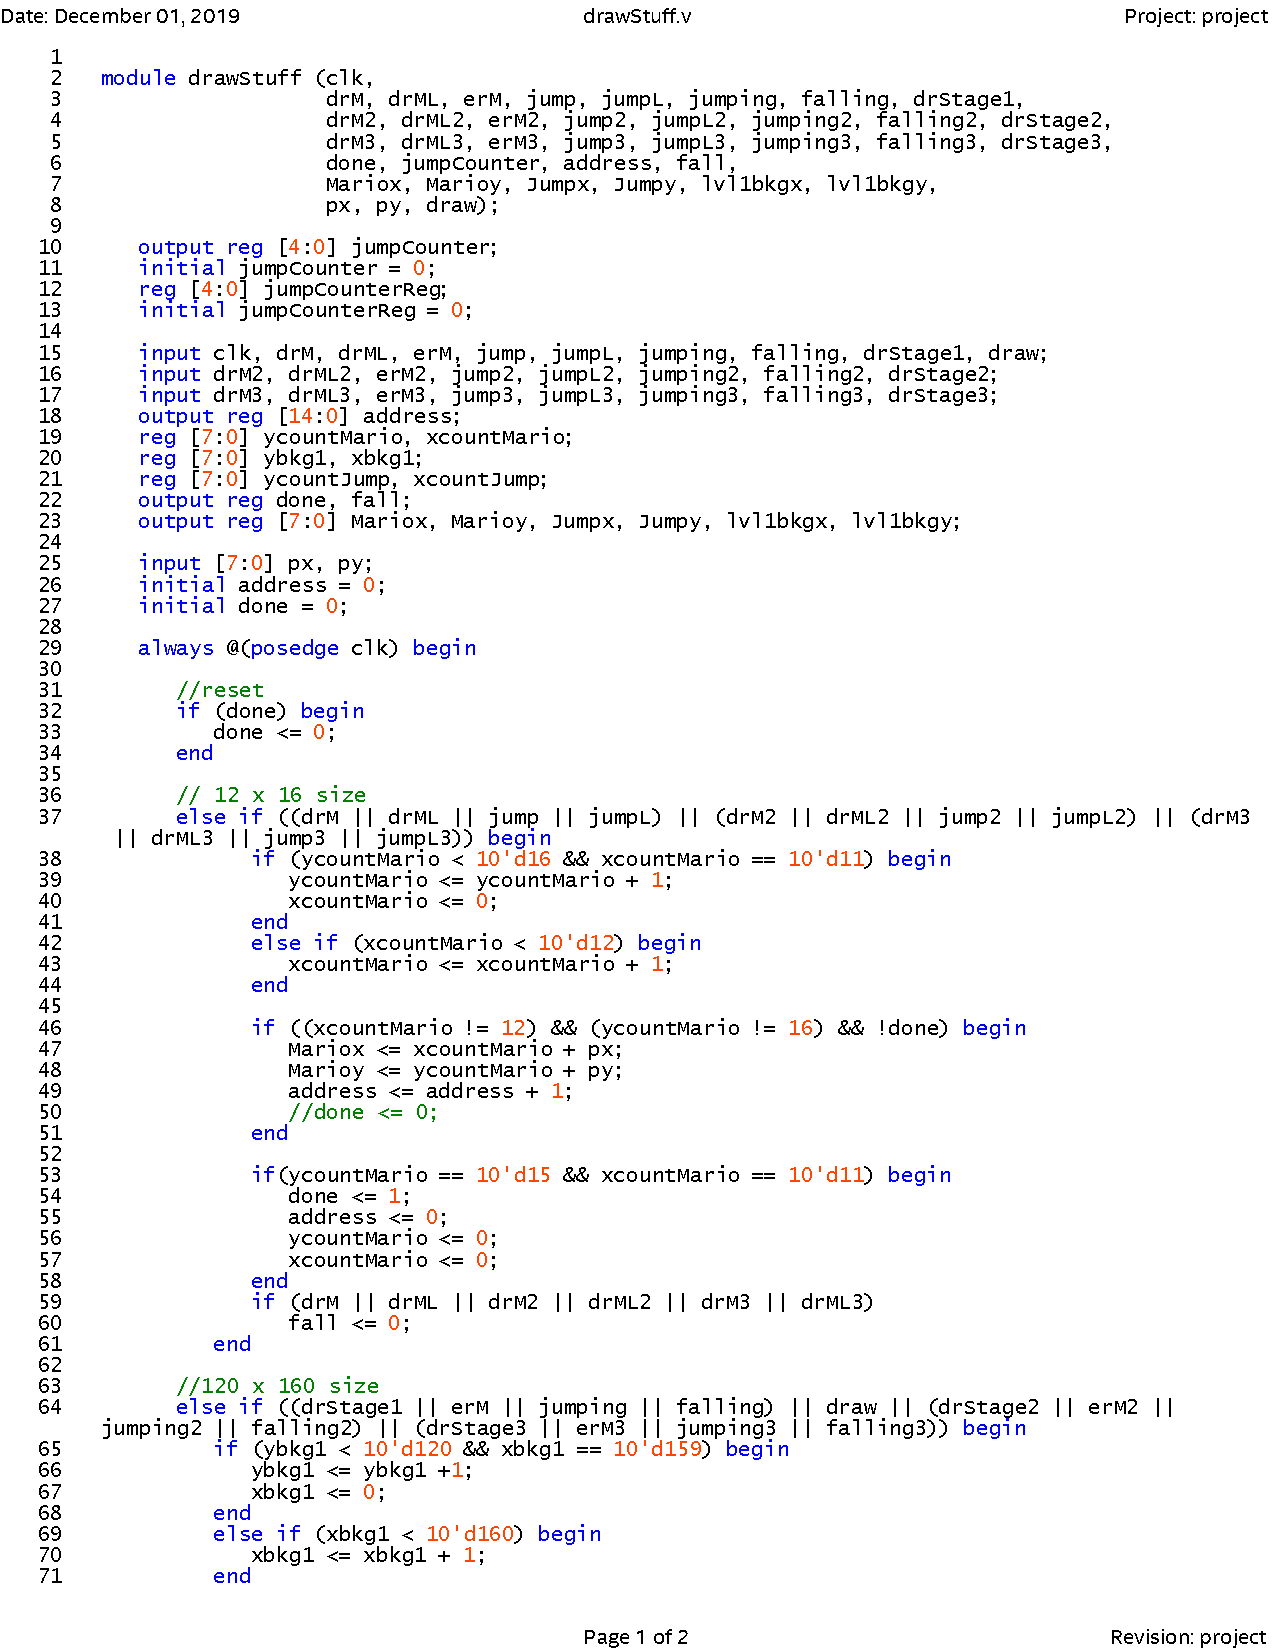
\includepdf[page=-]{4}
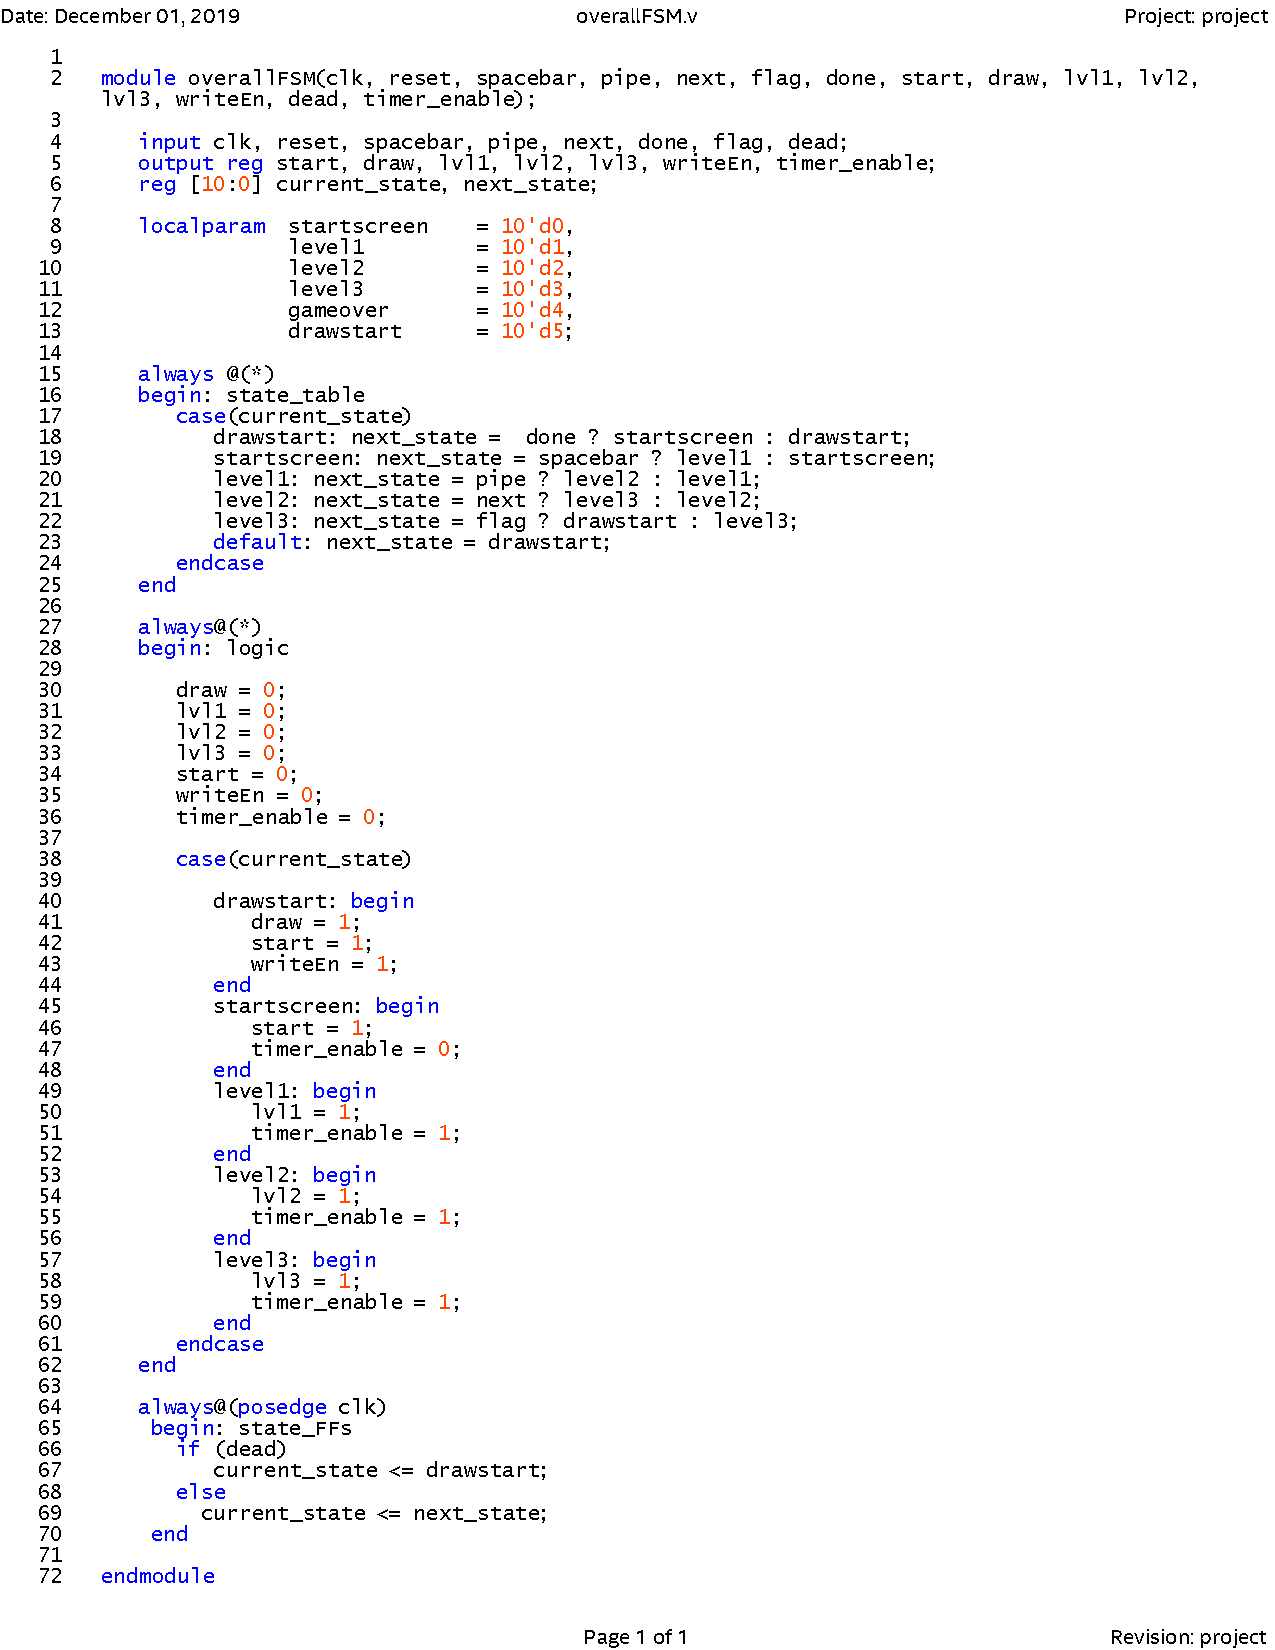
\includepdf[page=-]{5}
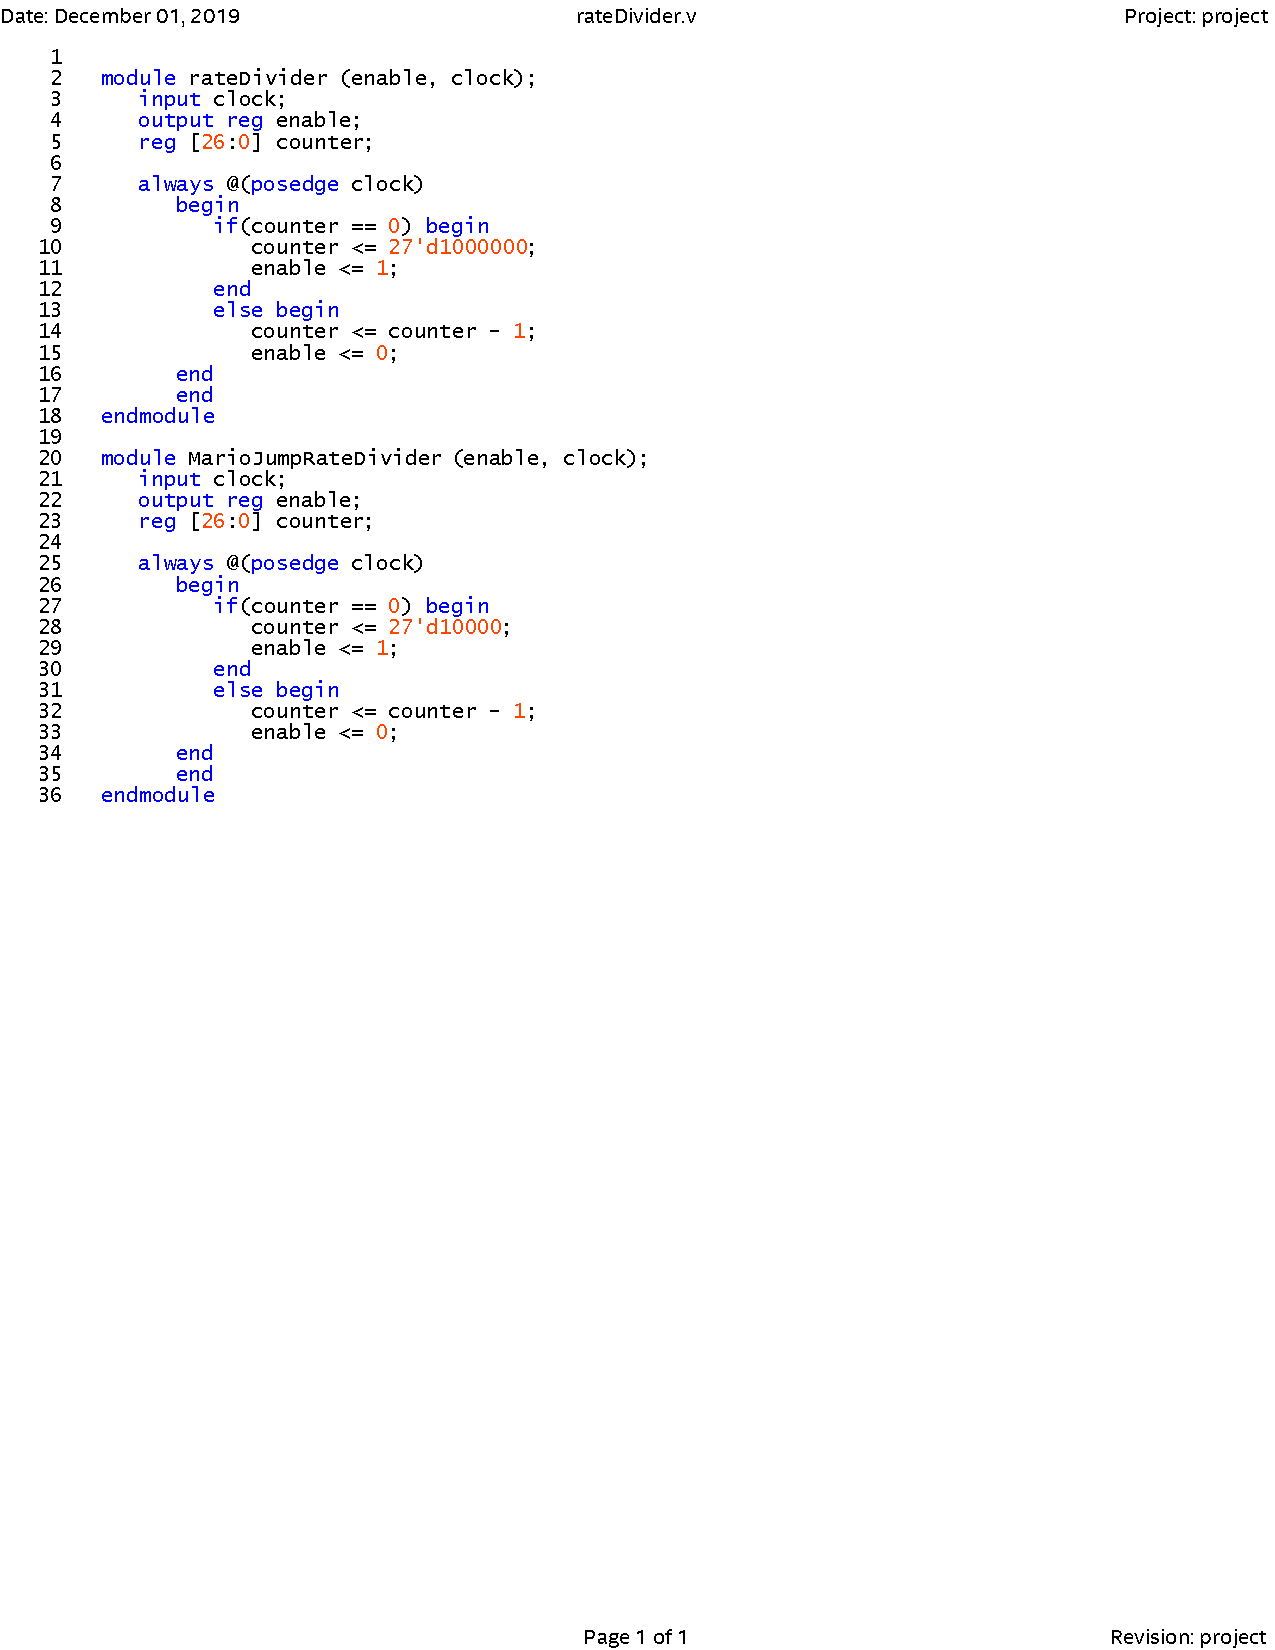
\includepdf[page=-]{6}

\end{document}


